\chapter{研究方法}
\fontsize{12pt}{18pt}\selectfont

% ------------------------- 3.0 ------------------------- %
% 研究目的;研究假設;研究方法
本研究目的是透過最佳化方法估計肌肉參數,省去醫療器材量測之高成本,藉以生成個人化模型,
應用於復健規劃、運動訓練與輔具設計等領域。本研究假設為已知一肌肉骨骼模型,該模型除了欲評估之肌肉參數外,
其餘幾何特徵、肌肉參數等資訊皆為已知,而其可透過 OpenSim 軟體來執行任何模擬。研究方法主要分為三大主軸,
介紹如下:
\begin{itemize}
    \item \textbf{主軸一:敏感度分析}
    \\ 透過擾動肌肉參數,來計算出任務與參數間之敏感度,其指標是藉由預測任務之誤差來表示。
       敏感度高意味著該肌肉和該任務具有高相關性,其結果提供最佳化與模型驗證之任務挑選的參考依據。
    \item \textbf{主軸二:多運動軌跡預測最佳化}
    \\ 從敏感度分析挑選數個適當任務作為輸入,並將多運動軌跡預測任務之平均預測誤差視作目標函數,
       藉由最佳化方法最小化平均預測誤差,以此估計出最佳模型之肌肉參數。   
    \item \textbf{主軸三:模型驗證}
    \\ 從敏感度分析挑選適當任務作為輸入,指定最佳模型完成並檢視其預測誤差,
       確認該模型是否於其它任務仍具有低誤差表現,以此驗證模型正確性。
\end{itemize}

% 研究流程圖 + 說明
本研究之流程圖如圖 所示,首先輸入標準模型和分析參數來執行敏感度分析,
藉由全因子實驗設計法來評估出所有任務之敏感度指標,接下來挑選適合的組合集作為最佳化之評估任務,
以生成最佳模型,最終透過高敏感度任務進行模型驗證,來評估最佳模型之正確性。
若於模型驗證階段成功,代表評估正確,並結束程式執行;若於模型驗證階段失敗,則返回至最佳化步驟重新評估;
若模型驗證失敗次數過多,則返回至敏感度分析流程,重新挑選合適的評估任務。
程式碼將發布於 https://github.com/solab-ntu/MuscleParamEstimation 該網址中,執行細節可檢視程式碼中的註解說明。

\clearpage

% ------------------------- 3.1 ------------------------- %
\section{實驗系統設定與實驗環境}\label{ch3_exp_setting}
% 系統架設;實驗環境
% 說明會講到實驗流程、系統設定、實驗環境等等的事情
進行人體姿勢估計實驗時,需要使用多種感測器來量測人體姿態,且需要多項事前準備工作及設置,
本章節將會依序說明整體實驗流程、室內室外實驗環境、實驗系統設定及實驗動作。

\subsection{實驗流程}
% 講我蒐集資料的事前工作,和整個流程的概述
在進行人體姿態估計的實驗流程如圖~\ref{ch3_fig_exp_flow} 所示,
首先進行相機內部參數及外部參數拍攝,
拍攝內部參數影片時,需使棋盤格校正板盡可能填滿畫面,並涵蓋多種不同角度的畫面,以便進行內部參數校正,
拍攝外部參數影片時,需由受試者站在實驗初始位置並拿著棋盤格校正板,以便進行外部參數校正。
接著進行個人化三維人體模型資料蒐集,
由受試者站在實驗初始位置,進行時間對齊動作後,維持 T pose 約 1 \textasciitilde\ 2 秒進行拍攝及 IMU 量測,最後再進行一次時間對齊動作,
完成個人化三維人體模型資料蒐集。
再來即可開始進行實驗動作資料蒐集,
由受試者站在實驗初始位置,進行時間對齊動作後,進行實驗動作拍攝及 IMU 量測,最後再進行一次時間對齊動作,
完成實驗動作資料蒐集。
實驗資料蒐集到此告一段落,接著將蒐集到的影像資料及 IMU 量測資料進行時間對齊、空間對齊,並進行感測器融合,
輸出即為立體人體姿態估計結果,最後計算肢段長度進行驗證。

\begin{figure}[!ht]
   \centering
   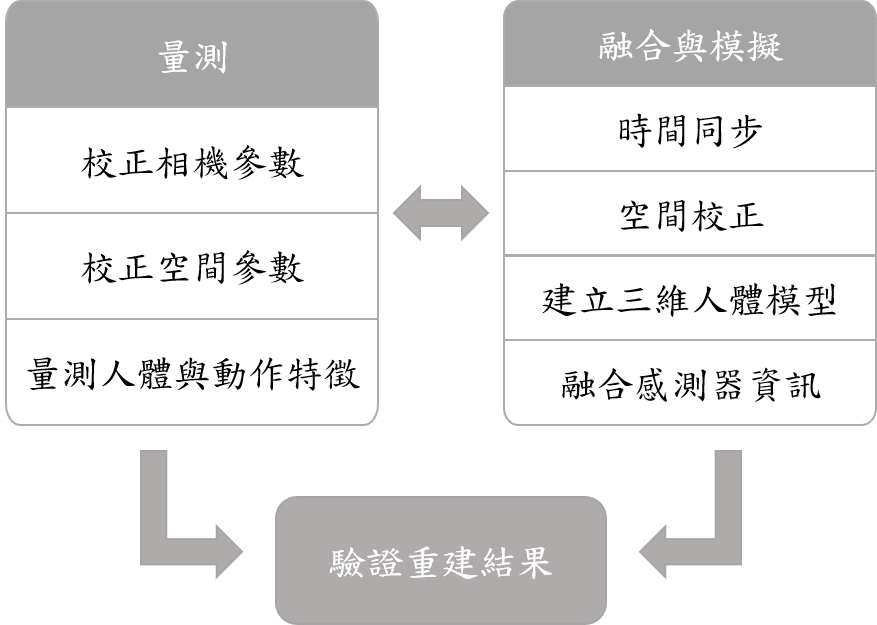
\includegraphics[width=\linewidth]{figure/ch3_fig_exp_flow.png}
    \caption[人體姿態估計實驗流程]{人體姿態估計實驗流程}
    \label{ch3_fig_exp_flow}
\end{figure}

% \subsection{實驗環境}
% % 實驗環境介紹
% 使用室內和室外環境,分開介紹

\subsection{室內實驗環境及尺寸}
% 室內實驗環境介紹
室內實驗環境空間尺寸為 880$\times$880 (cm),全室拉上遮光布遮蔽室外光線,
量測時間為晚上 8 點至 9 點,以確保環境光線穩定,並減少環境光對影像資料的影響。
實驗環境及尺寸如圖~\ref{ch3_fig_indoor_scale} 所示,
受試者初始位置為圖中黑色空心圓圈位置,實驗過程中於 278$\times$283 (cm) 的方形範圍內進行動作,
用於錄製影像的兩台手機位置於圖~\ref{ch3_fig_indoor_scale}中紅點標示處。
實際實驗環境及受試者位置如圖~\ref{ch3_fig_indoor_position} 所示。

\begin{figure}[!ht]
   \centering
   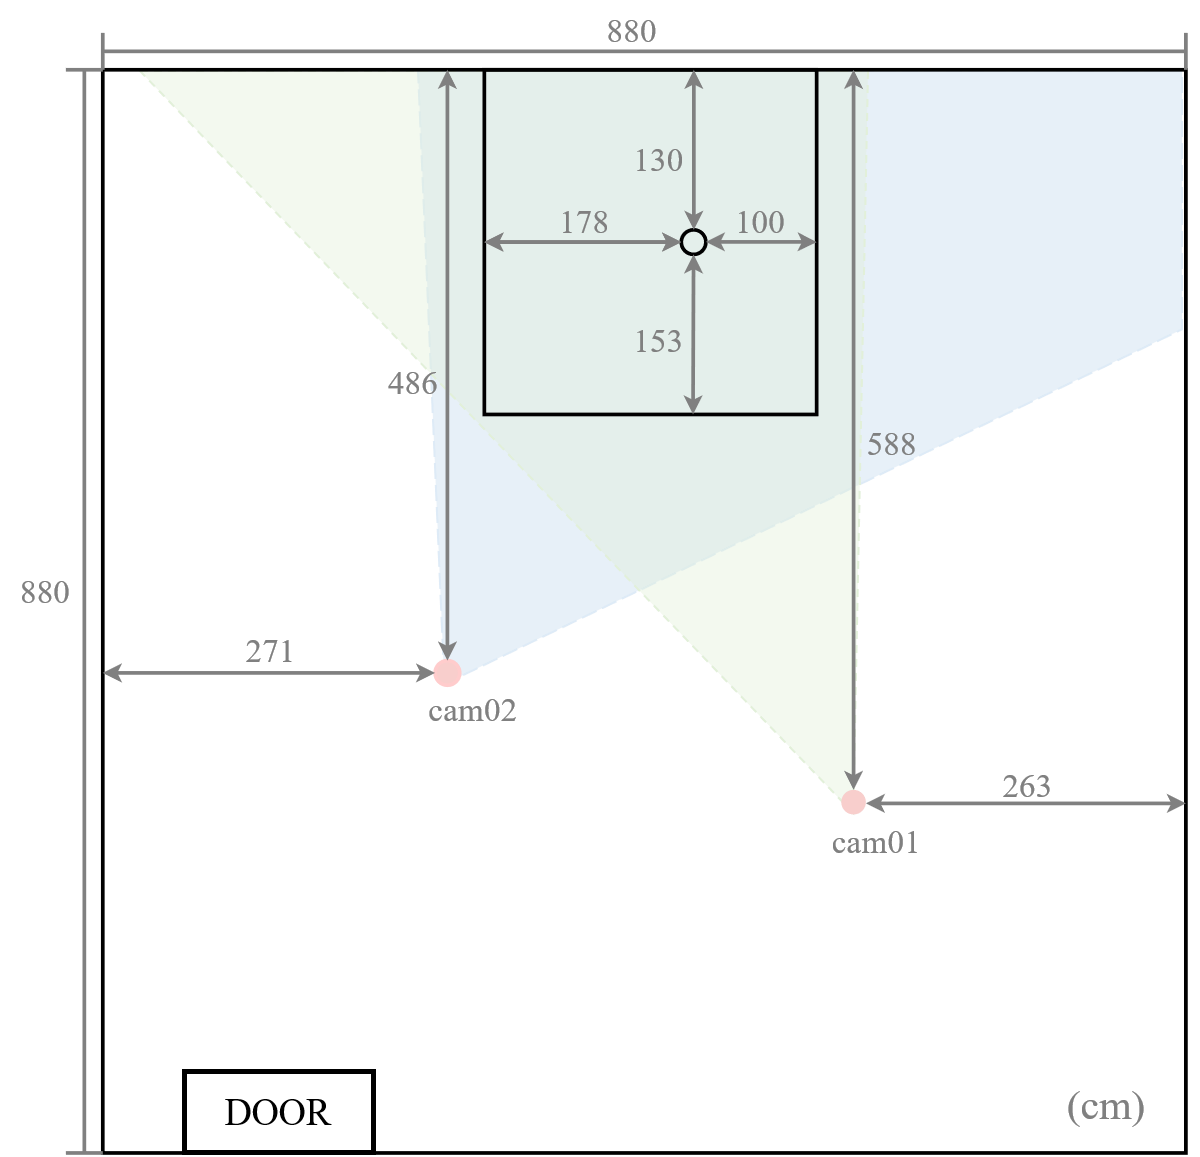
\includegraphics[width=\linewidth]{figure/ch3_fig_indoor_scale.png}
    \caption[室內實驗環境及尺寸]{室內實驗環境及尺寸}
    \label{ch3_fig_indoor_scale}
\end{figure}

\begin{figure}[!ht]
   \centering
   \begin{minipage}{.5\textwidth}
     \centering
     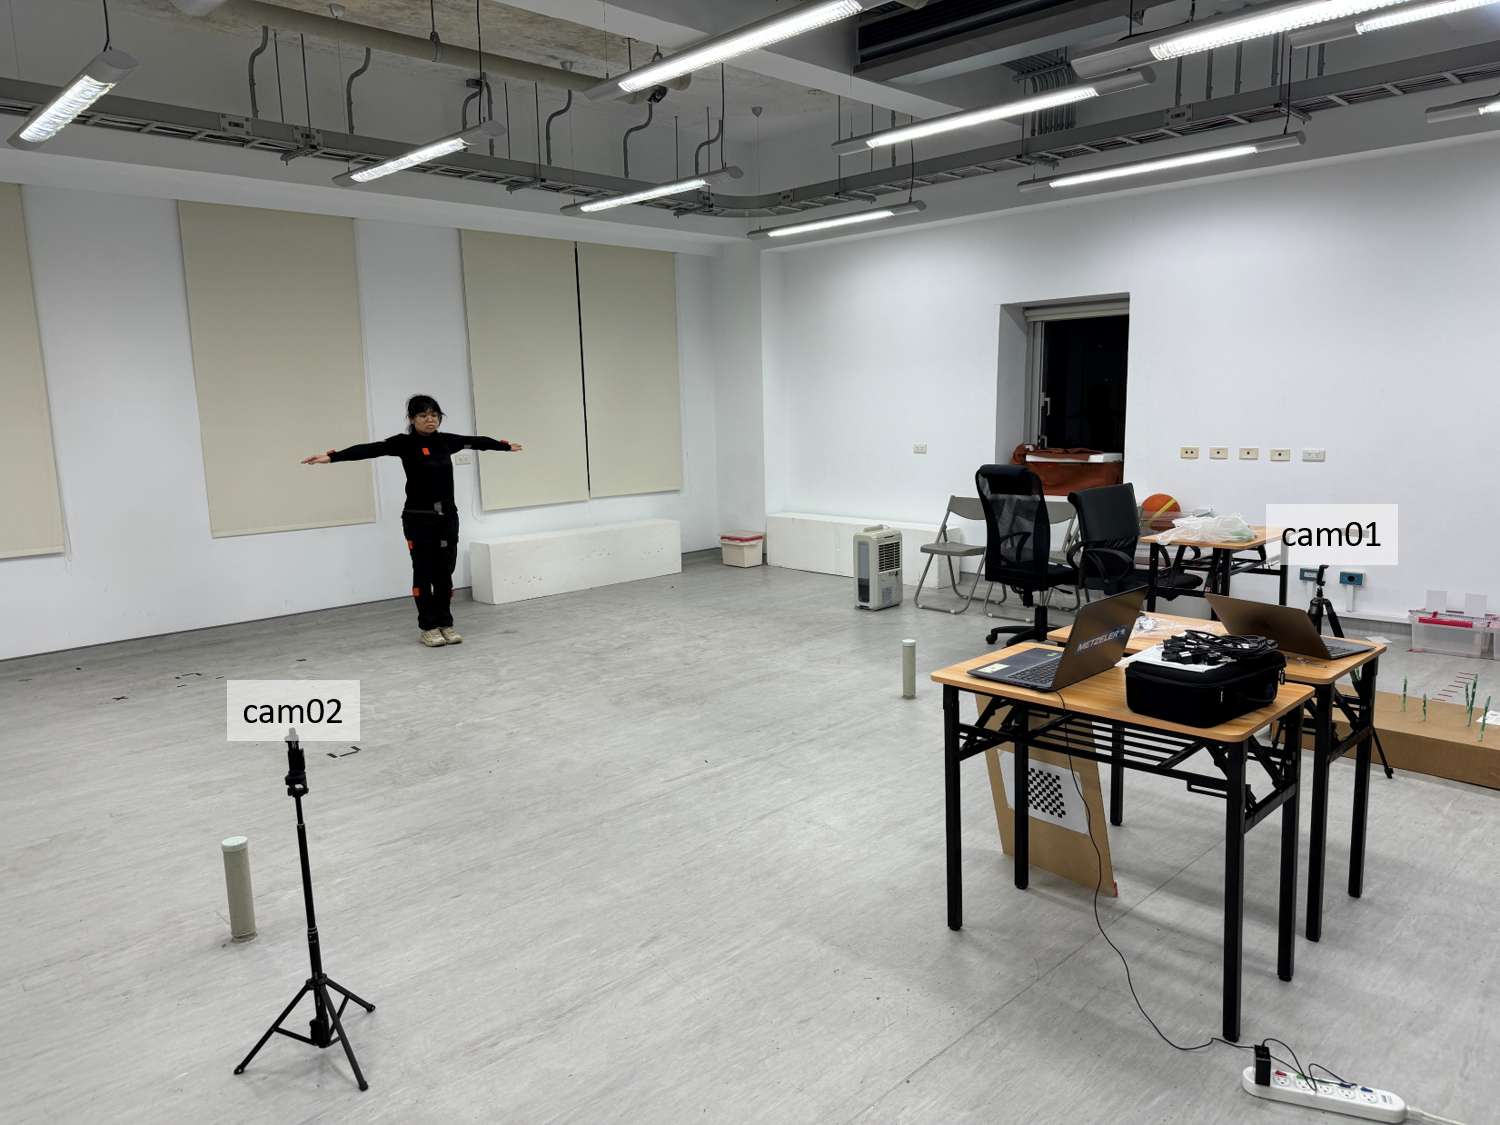
\includegraphics[width=\linewidth]{figure/ch3_fig_indoor_position1.png}
     \caption*{(a)相機與受試者位置 (前視)}
   \end{minipage}%
   \begin{minipage}{.5\textwidth}
      \centering
      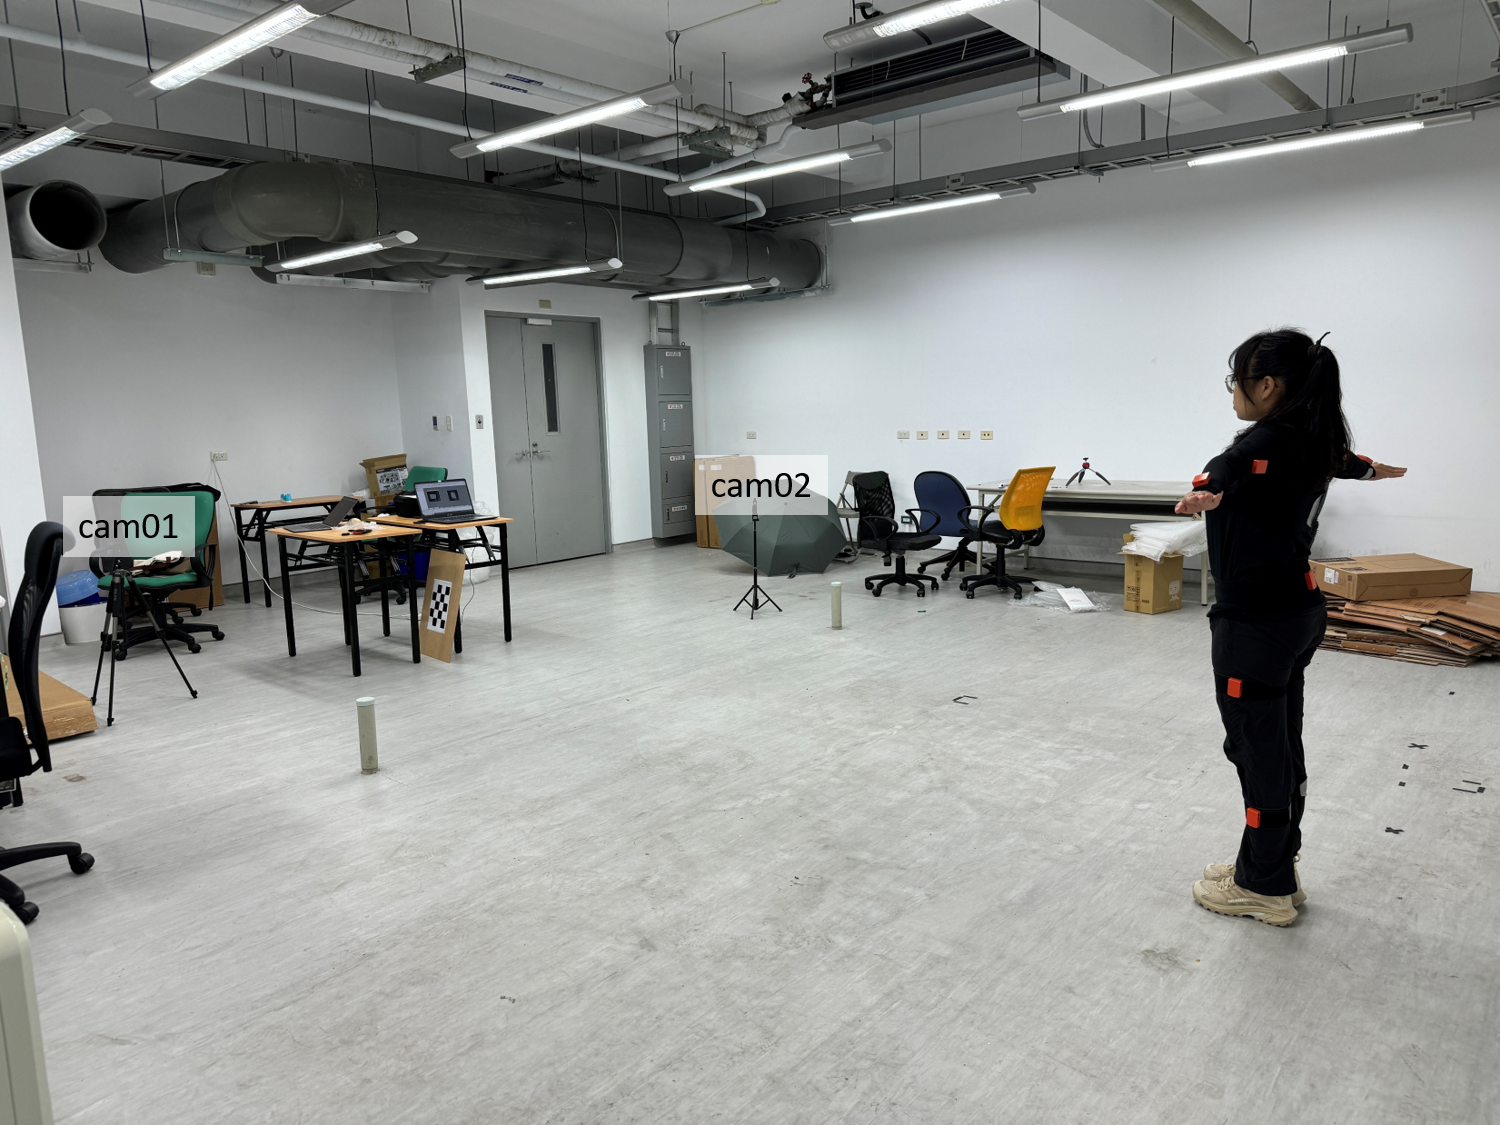
\includegraphics[width=\linewidth]{figure/ch3_fig_indoor_position2.png}
      \caption*{(b)相機與受試者位置 (後視)}
   \end{minipage}%
   \caption[室內實際實驗環境及相機與受試者位置]{室內實際實驗環境及相機與受試者位置}
   \label{ch3_fig_indoor_position}
\end{figure}

\subsection{室外實驗環境及尺寸}
% 室外實驗環境介紹
% 這邊可以放一張室外實驗環境的照片
所有房間尺寸、活動範圍尺寸、相機位置和高度

\subsection{實驗系統設定}
% 系統架設介紹
本研究用於量測人體姿態的工具包含兩台 iPhone 手機、Xsens、棋盤格校正板。
兩台手機用於記錄人體姿態的影像資料,擺放於固定位置、固定角度,拍攝受試者的全身影像;
Xsens 用於記錄人體各肢段及棋盤格校正板的朝向資訊,共使用 10+1 顆 IMU 進行量測;
棋盤格校正板用於進行相機校正,取得相機內部參數及外部參數,以建立影像座標系與全域座標系間的關係。
另外,需要求受試者穿著黑色長袖上衣及黑色長褲,長度盡可能遮蓋住手腕及腳踝。


\subsubsection{位置資訊量測工具 - 相機及擺放位置}
本研究使用兩支 iPhone 手機進行影像資料蒐集,分別為 iPhone XR 及 iPhone 15 Pro,
iPhone XR 使用主鏡頭進行拍攝,焦距 26 (mm),光圈 ƒ/1.8,iPhone 15 Pro 使用主鏡頭進行拍攝,焦距 24 (mm),光圈 ƒ/1.78,
兩支手機皆設定影像擷取畫面為 1920x1080,幀率設定為 60 Hz。

% FIXME:環境有室內環境和室外環境,這邊有必要分開描述,但要再想想該如何描述
本研究將 iPhone XR 編號為 cam01,將 iPhone 15 Pro 編號為 cam02,
手機擺放位置為圖~\ref{ch3_fig_indoor_scale} 中紅色圓點處,cam01 拍攝高度為 79 (cm),cam02 拍攝高度為 74 (cm),
cam 01 的拍攝視角為圖~\ref{ch3_fig_indoor_scale} 中綠色範圍,cam 02 的拍攝視角為圖~\ref{ch3_fig_indoor_scale} 中藍色範圍,
在實驗資料蒐集過程中,拍攝角度及位置皆維持不變。

\subsubsection{朝向資訊量測工具 - Xsens}
本研究使用 Xsens 提供之硬體及軟體 MT-manager 作為量測姿態朝向的工具,採樣率設定為 60 Hz,共使用 10+1 顆 IMU 進行量測,
十顆 IMU 分別黏貼於左右上臂中段外側、左右手腕外側、胸骨、骨盆、左右大腿中段外側、左右小腿中段外側,共十處,
如圖~\ref{ch3_fig_humanimu} 所示, IMU 長軸 (即 x 軸) 與骨頭長度方向對齊,隨時間進行蒐集各時間點受試者各肢段的朝向資訊。
另一顆 IMU 黏貼於棋盤格校正板,量測棋盤格校正板的初始朝向,用以轉換影像座標系至全域座標系,如圖~\ref{ch3_fig_imgimu} 所示,
IMU 的 x、y 軸方向對齊棋盤格校正板的 x、y 座標方向。

\begin{figure}[!ht]
   \centering
   \begin{minipage}{.25\textwidth}
     \centering
     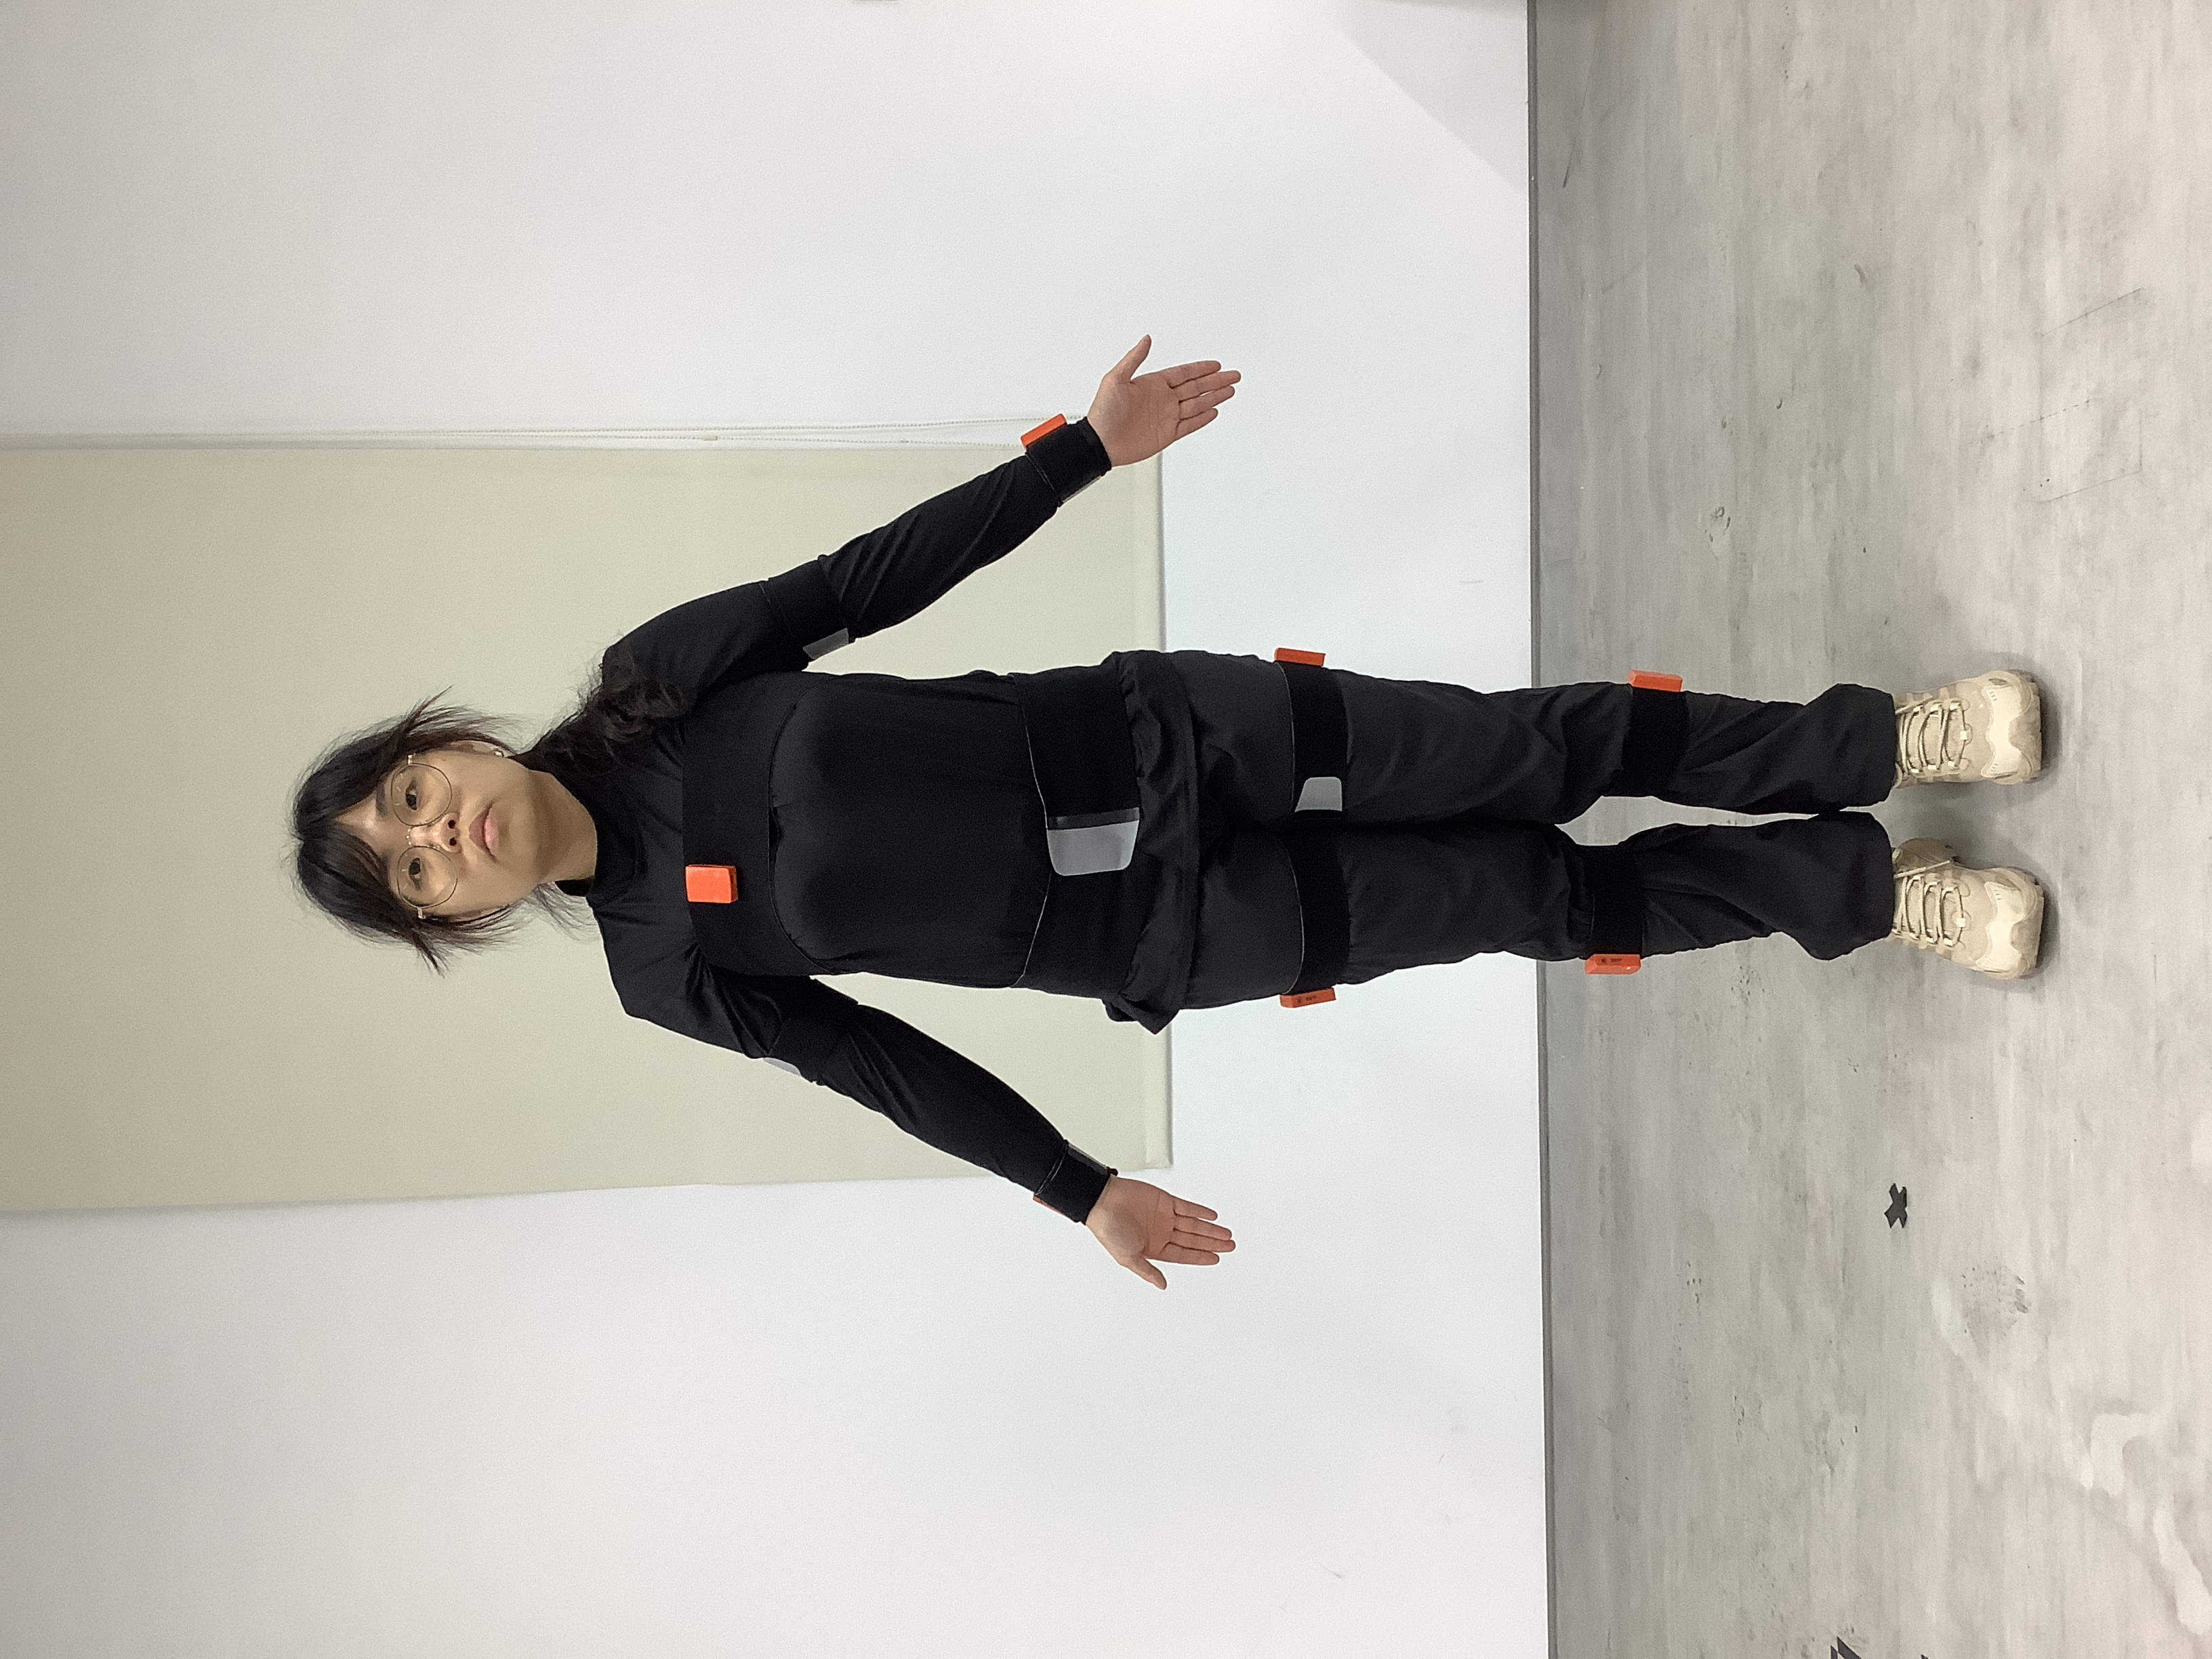
\includegraphics[width=\linewidth, angle=-90]{figure/ch3_fig_frontimu.JPG}
     \caption*{(a) 前視}
   \end{minipage}%
   \begin{minipage}{.25\textwidth}
      \centering
      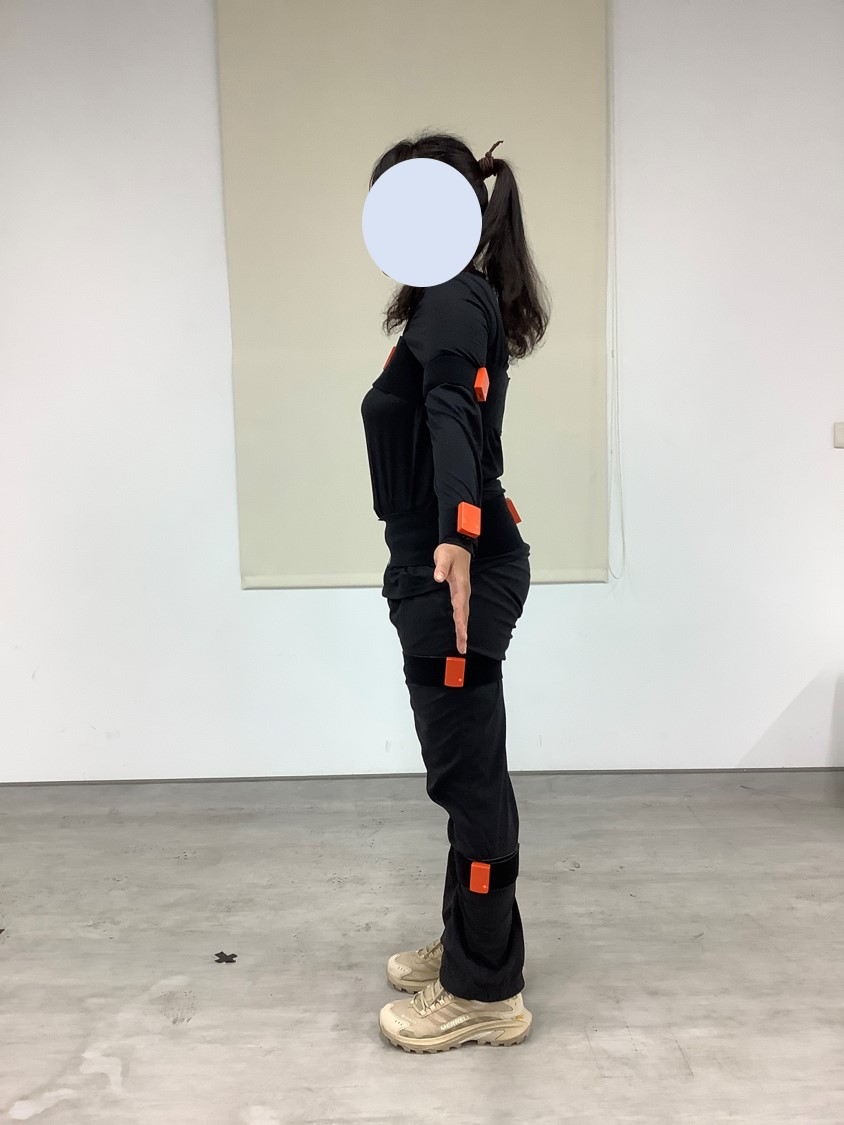
\includegraphics[width=\linewidth, angle=-90]{figure/ch3_fig_leftimu.JPG}
      \caption*{(b) 左視}
   \end{minipage}%
   \begin{minipage}{.25\textwidth}
      \centering
      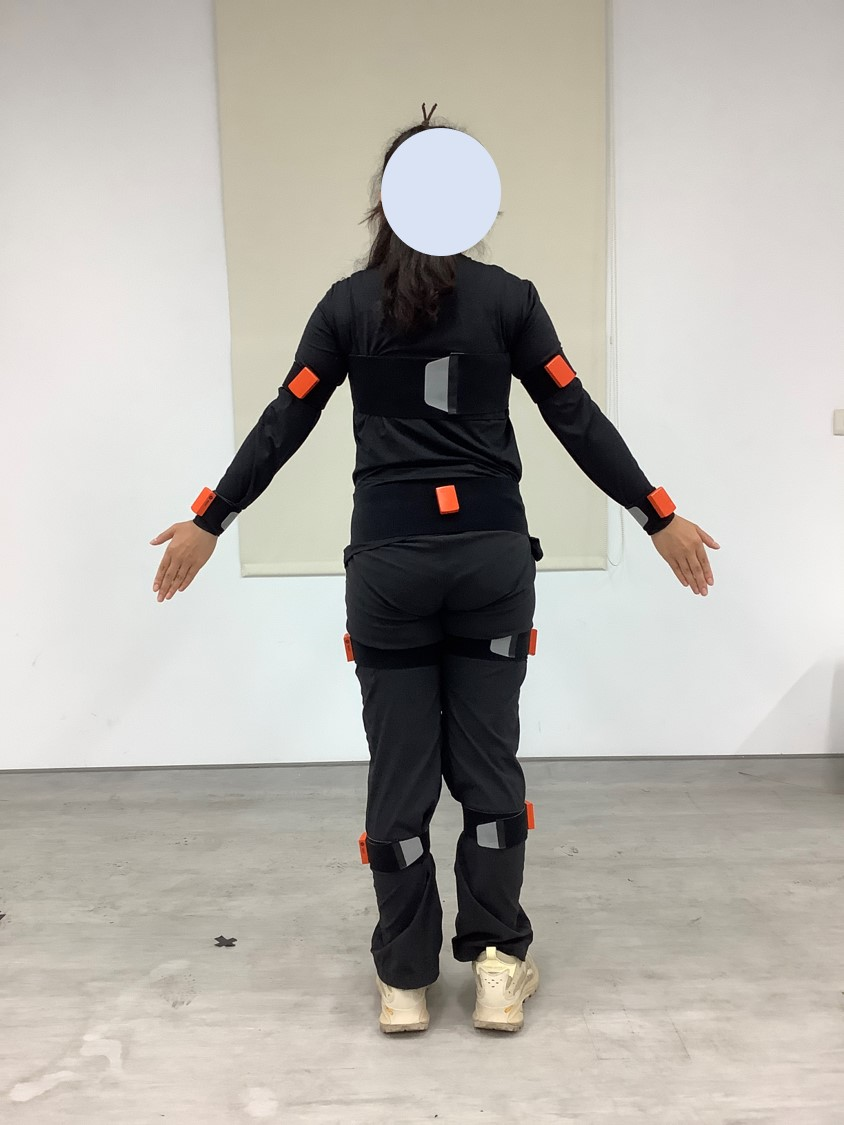
\includegraphics[width=\linewidth, angle=-90]{figure/ch3_fig_backimu.JPG}
      \caption*{(c) 後視}
   \end{minipage}%
   \begin{minipage}{.25\textwidth}
     \centering
     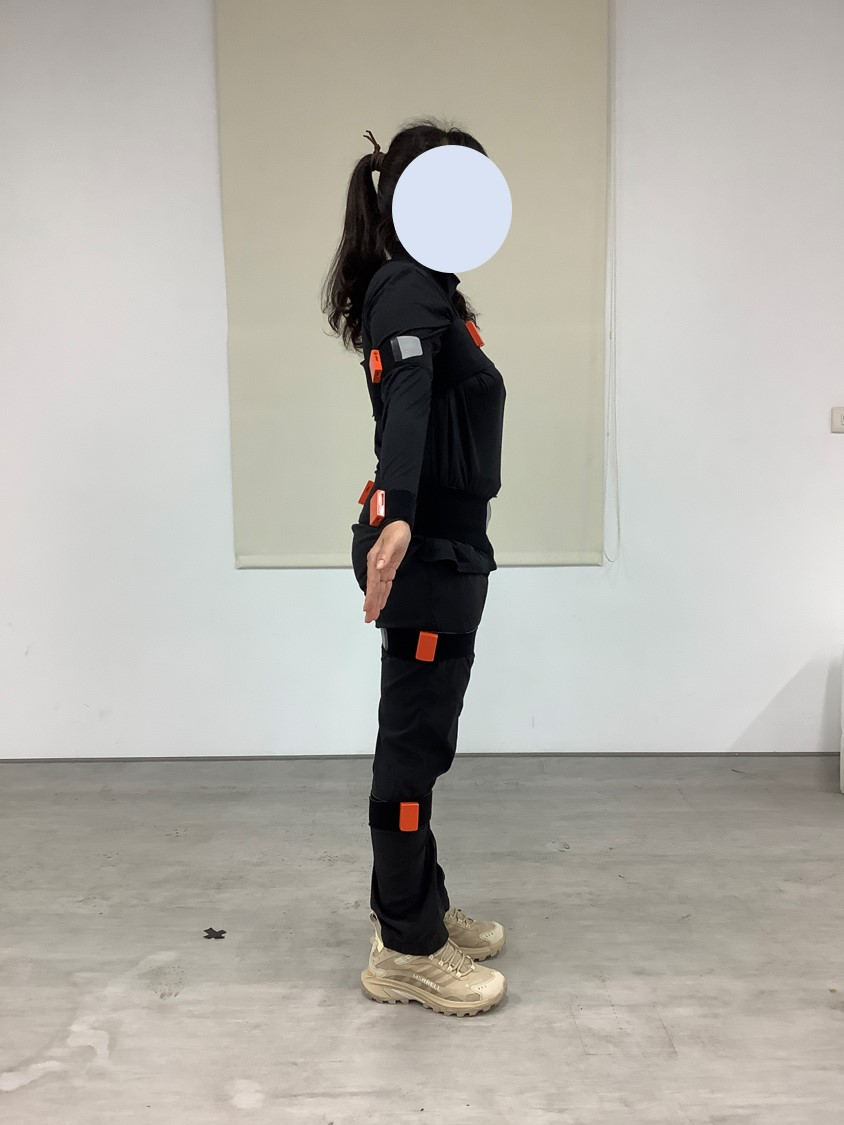
\includegraphics[width=\linewidth, angle=-90]{figure/ch3_fig_rightimu.JPG}
     \caption*{(d) 右視}
   \end{minipage}
   \caption[IMU 於人體黏貼位置及方向]{IMU 於人體黏貼位置及方向}
   \label{ch3_fig_humanimu}
\end{figure}

\begin{figure}[!ht]
   \centering
   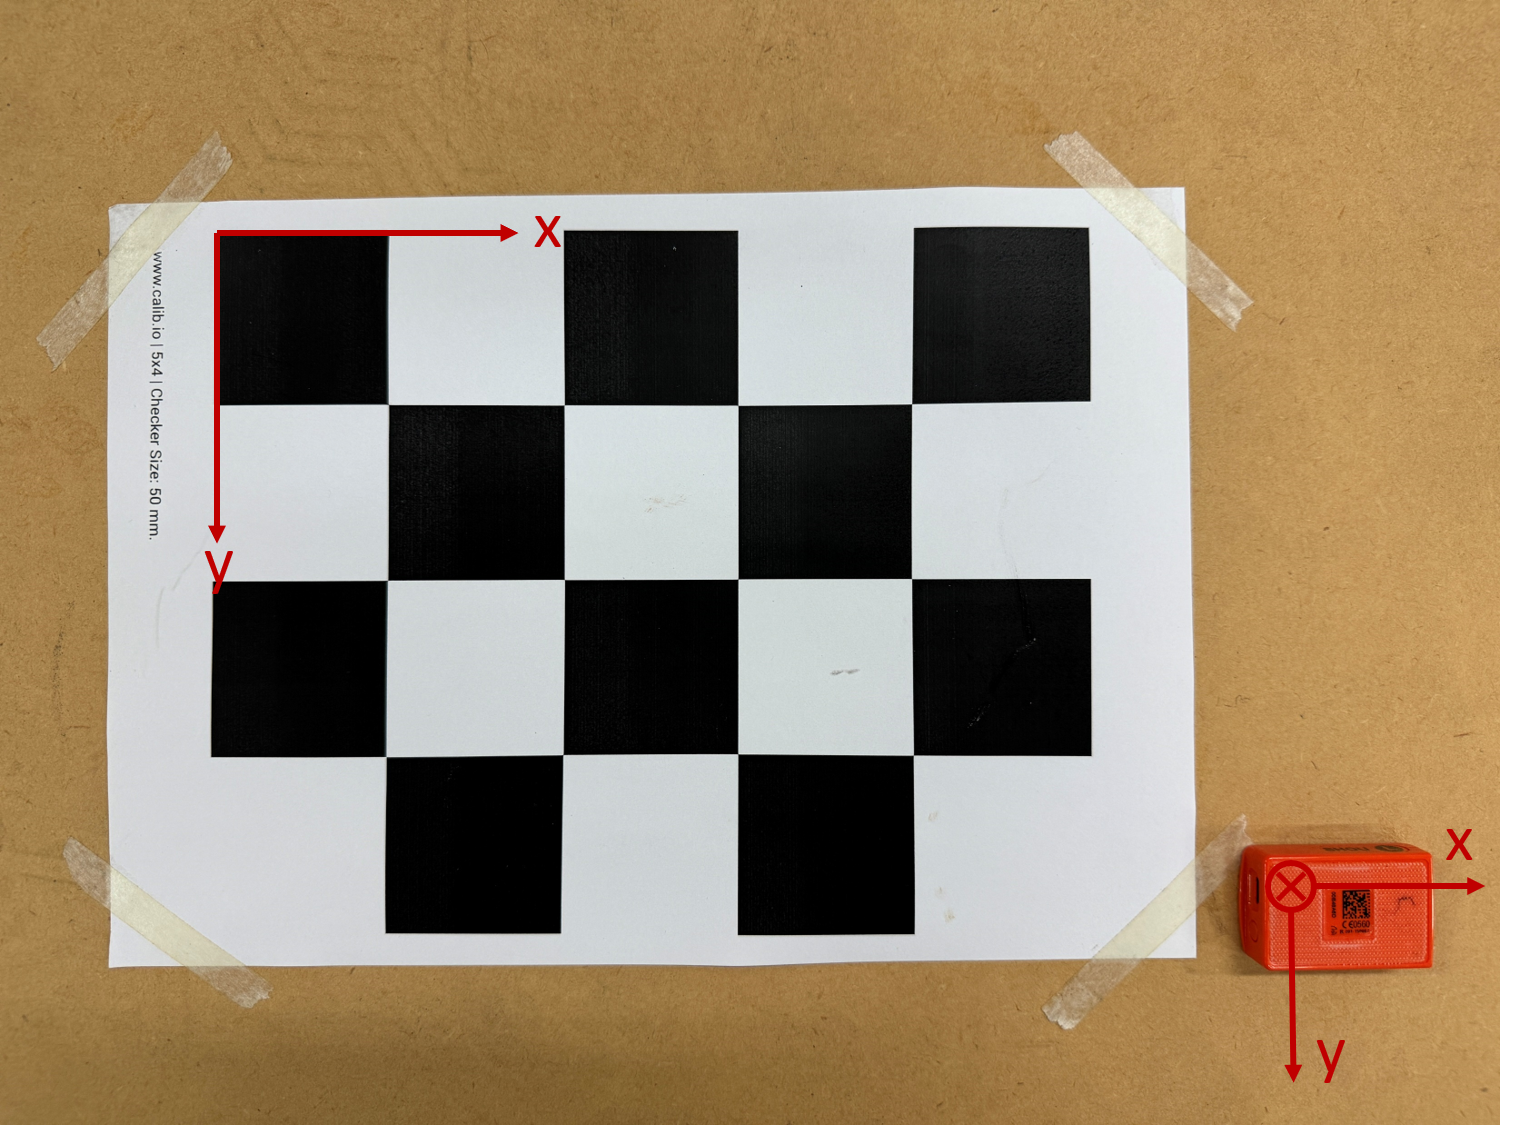
\includegraphics[width=8cm]{figure/ch3_fig_imgimu.png}
    \caption[IMU 於棋盤格校正板黏貼位置及方向]{IMU 於棋盤格校正板黏貼位置及方向}
    \label{ch3_fig_imgimu}
\end{figure}

\subsection{實驗動作}
% 實驗動作介紹
現在還不確定要不要把每個動作的量測目的都寫出來,畢竟結果也不好

% ------------------------- 3.2 ------------------------- %
\section{資料前處理}
% 資料前處理介紹
% 利用章節~\ref{ch3_exp_setting} 介紹的系統蒐集完實驗資料後,接下來將進行資料前處理,以利後續進行感測器融合。
% 資料前處理分為個人化人體模型建立、獲取骨盆中點位置、時間對齊、空間對齊四個部分,將於本章節進行討論。

\subsection{相機校正}
相機校正可視為影像世界和真實世界之間的轉換,其中包含外部參數 (Extrinsic Parameter) 及內部參數 (Intrinsic Parameter) 兩部分,
透過相機校正計算公式~\ref{ch3_equ_camera_calibration},可以將全域座標系中的點轉換成在影像座標系中的點,
如圖~\ref{ch3_fig_camera_calibration}所示,
將在全域座標系 (global coordinate system, g) 中的點 $P_g$,經過特定的旋轉、平移轉換及投影後,
就可以轉換成影像座標系 (image coordinate system, img) 中的點 $P_{img}$。

\begin{equation}
   s
   \begin{bmatrix}
      u \\ v \\ 1
   \end{bmatrix}
   =
   \begin{bmatrix}
      \alpha_x & s & u_o \\
      0 & \alpha_y & v_o \\
      0 & 0 & 1 \\
   \end{bmatrix}
   \begin{bmatrix}
      r_{11} & r_{12} & r_{13} & t_{1} \\
      r_{21} & r_{22} & r_{23} & t_{2} \\
      r_{31} & r_{32} & r_{33} & t_{3} \\
   \end{bmatrix}
   \begin{bmatrix}
      X \\
      Y \\
      Z \\
      1 \\
   \end{bmatrix}
   \label{ch3_equ_camera_calibration}
\end{equation}

\begin{figure}[!ht]
   \centering
   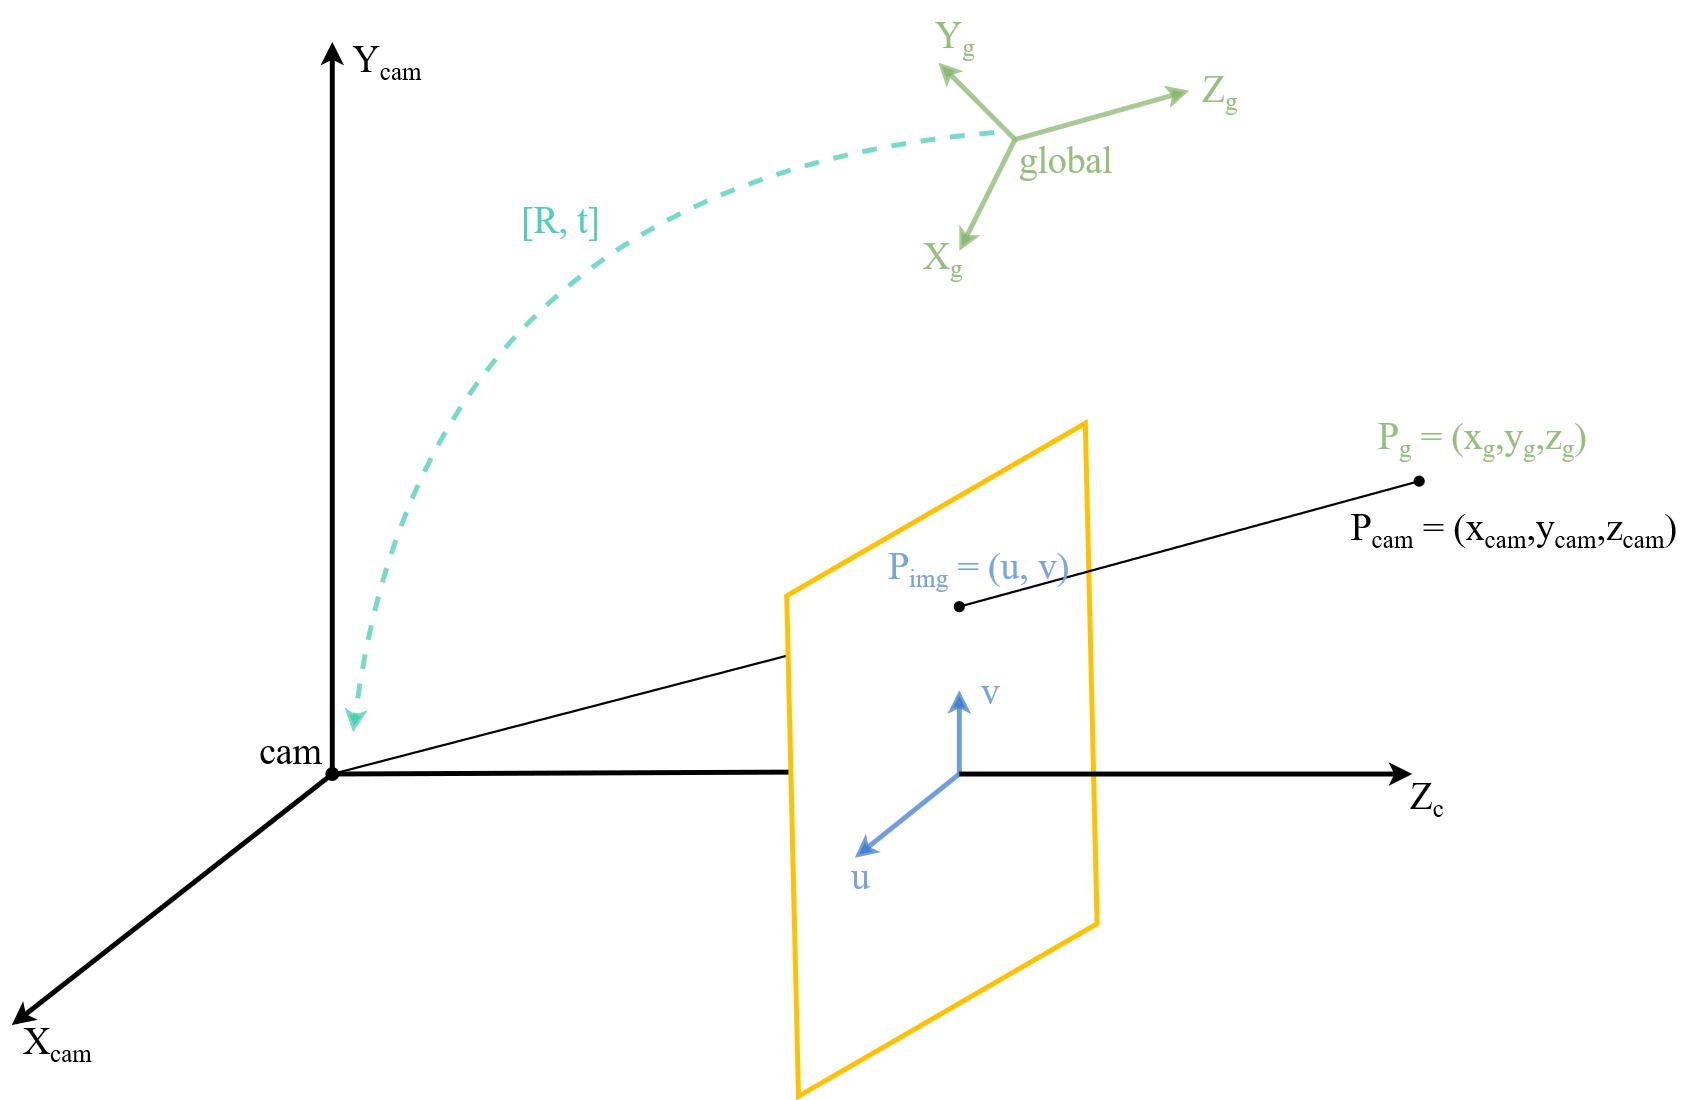
\includegraphics[width=\linewidth]{figure/ch3_fig_camera_calibration.png}
    \caption[相機校正座標系~\cite{dehkharghani2014geometric}]{相機校正座標系~\cite{dehkharghani2014geometric}}
    \label{ch3_fig_camera_calibration}
\end{figure}

\subsubsection*{外部參數}
如圖~\ref{ch3_fig_camera_calibration},
假設有一在原點為校正板左上角的全域座標系 (global coordinate system, g) 中的點 $P_g$,
將 $P_g$ 經過特定的旋轉及平移轉換後,就可以轉換成以相機焦點為原點的相機座標系 (camera coordinate system, cam) 中的點 $P_{cam}$,
這個特定的旋轉及平移轉換即為相機的外部參數,旋轉以一個 3$\times$3 的旋轉矩陣 $R$ 表示,平移以一個 3$\times$1 的平移向量 $T$ 表示,
因為在矩陣計算上,世界座標會先經過旋轉再平移,因此平移向量 $T$ 會經過旋轉矩陣 $R$ 的作用,形成 $RT$,
再將 $[R|RT]$ 合併形成一個 3$\times$4 的外部參數矩陣 $[R|RT]$,
即為式~\ref{ch3_equ_camera_calibration}中,等號右邊第二項。

\subsubsection*{內部參數}
將在相機座標系中的點 $P_{cam}$ 經過投影、平移及幾何校正,轉換成在影像座標系 (image coordinate system) 中的點為 $P_{img}$,
為圖~\ref{ch3_fig_camera_calibration}中,將 $P_{cam}$ 轉換至 $P_{img}$ 的過程,
這個投影、平移及幾何校正的過程即為相機的內部參數,為一個 3$\times$3 的矩陣,
即為式~\ref{ch3_equ_camera_calibration}中,等號右邊第一項,
內部參數包含焦距、影像座標系的圓點位置、解析度、 pixel 夾角等參數,
由於這些參數皆與相機內部的硬體參數有關,因此稱為相機內部參數。

\subsection{個人化三維人體模型建立}\label{ch3_skeleton_method}
% 個人化三維人體模型建立介紹
% 伸縮沒有寫到,要怎麼加進去?
% TODO:覺得可以把我為甚麼選擇用 OpenPose 不用 mediapipe 寫在這邊
% FIXME:通用模型轉成個人化模型,要補上這邊的人體模型是為了讓 IMU 建立人體姿態
在文獻~\cite{Zhang_2020_CVPR} 中,作者使用 Vicon 系統所提供的三維人體模型,
並以其為基礎,進行 IMU 計算;但是在非實驗室的環境中無法使用 Vicon 進行量測,進而取得三維人體模型。
因此本研究透過 Pose2Sim ~\cite{Pagnon_2022_JOSS}~\cite{Pagnon_2021_Robustness}~\cite{Pagnon_2022_Accuracy} 提出之方法,
使用影像辨識技術,辨識每一視角中人體的關節點在影像中的位置,並利用相機校正技術建立出每一關節在空間中的位置,以此方式建立個人三維人體模型。

% 章節~\ref{ch4_skeleton_exp} 將會利用 TotalCapture Dataset~\cite{Trumble:BMVC:2017}提供的影像資料,進行影像辨識與三角測量計算,
% 並將結果與 TotalCapture Dataset 提供之 Vicon 三維人體模型比對,以驗證此方法的可行性。

\subsubsection{建立方法}
% 影像辨識
% 這邊好像跟第四章的4.1.1有點重複,如果這邊和4.1都要留的話可能就要把下一節的結果與驗證搬到4.1那邊
% 這邊就只要簡單介紹一下方法就好,然後這邊可以應該可以把為何要選 OpenPose 不選 mediapipe 也寫上去
% 只是這樣的話就要想一下4.1.2的實驗執行要怎麼寫(不然如果真的想不到可能就要刪掉實驗執行這塊,畢竟也只是 run 而已),
% 4.1.1的應該可以寫用了哪些數據
% 考慮要不要寫為何選擇使用 OpenPose 不選 mediapipe,要寫的話可以寫在這一段的開頭
本方法流程如圖~\ref{ch3_fig_skeleton_flow} 所示。
以 T pose 的姿勢拍攝影片後,進入後續軟體端處理流程。
首先,使用 OpenPose~\cite{8765346}~\cite{wei2016cpm}~\cite{simon2017hand}~\cite{cao2017realtime}
影像辨識技術辨識每一視角人體關節點在影像中的位置(使用 BODY-25B model),辨識結果如圖~\ref{ch3_fig_OpenPose_result} 所示,
% FIXME:想把這張圖改成用 T pose 辨識出來的圖
其可辨識出左右肩膀、左右手肘、左右手腕、左右骨盆、左右膝蓋、左右腳踝等關節位置,如圖~\ref{ch3_fig_OpenPose} 所示;
接著,利用棋盤格方法之相機校正技術計算出各個相機的內部參數及外部參數;
再來,利用方才相機校正之結果,經由三角測量計算建立出關節在空間中的位置,並使用距離公式計算每一關節之間的距離;
最後,基於 TotalCapture Dataset 提供之 vicon 三維人體模型,利用計算出的距離進行三維人體模型伸縮,
得到與受試者四肢、身高相似之個人化三維人體模型,如圖~\ref{ch3_fig_my_skeleton}。

\begin{figure}[!ht]
   \centering
   
\includegraphics[width=\linewidth]{figure/ch3_fig_skeleton_flow.png}
    \caption[個人化三維人體模型建立流程圖]{個人化三維人體模型建立流程圖}
    \label{ch3_fig_skeleton_flow}
\end{figure}

\begin{figure}[!ht]
   \centering
   \includegraphics[width=8cm]{figure/ch3_fig_OpenPose_result.png}
   \caption[OpenPose 辨識結果]{OpenPose 辨識結果}
   \label{ch3_fig_OpenPose_result}
\end{figure}

\begin{figure}[!ht]
   \centering
   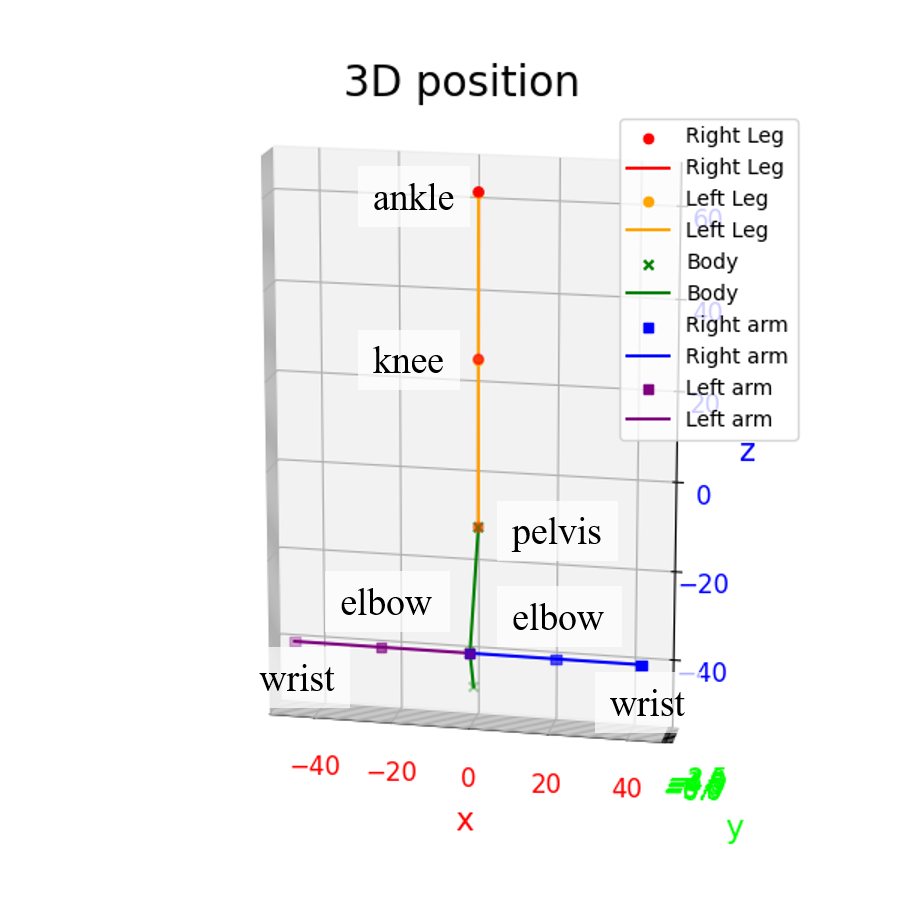
\includegraphics[width=8cm]{figure/ch3_fig_my_skeleton.png}
   \caption[個人化三維人體模型建立結果]{個人化三維人體模型建立結果}
   \label{ch3_fig_my_skeleton}
\end{figure}

\subsection{計算骨盆在影像中的像素位置}
% 軟體介紹;OpenPose
% OpenPose 為一款
% 由  Ginés Hidalgo, Zhe Cao, Tomas Simon, Shih-En Wei, Yaadhav Raaj, Hanbyul Joo, and Yaser Sheikh 等人開發的開源軟體,
% 為第一個在單個圖像上可以同時偵測人體關節、手部關節、面部表情和足部關鍵點(總共 135 個關鍵點)的實時多人偵測系統,
% 其可於 Windows、MacOS、Ubuntu 等作業系統上執行,並支援 Python、C++ 等程式語言,
% 輸入資源包括圖片、影像、網路攝影機等,
% 並可輸出原始影像加關鍵點顯示的疊圖 (PNG,JPG,AVI,...),
% 或是輸出純文字檔案 (JSON,XML,YAML...),其中紀錄關鍵點相對於輸入圖像的像素座標位置及 0~1 的分數。
% FIXME:在fusing wearable 中用 vicon 和相機參數轉換到影像坐標系,在進行裁切
本研究使用 OpenPose 作為影像辨識工具,搭配其提供之 BODY\_25B 模型進行影像辨識,
辨識出每一幀照片中 25 個人體關鍵點在圖像中的像素位置,可辨識出的關鍵點如圖~\ref{ch3_fig_OpenPose} 所示,
並進一步計算左骨盆及右骨盆的中點在圖像中的像素位置,以此計算結果作為該張影像的中點進行畫面裁切,減低後續感測器融合的計算量。

\begin{figure}[!ht]
   \centering
   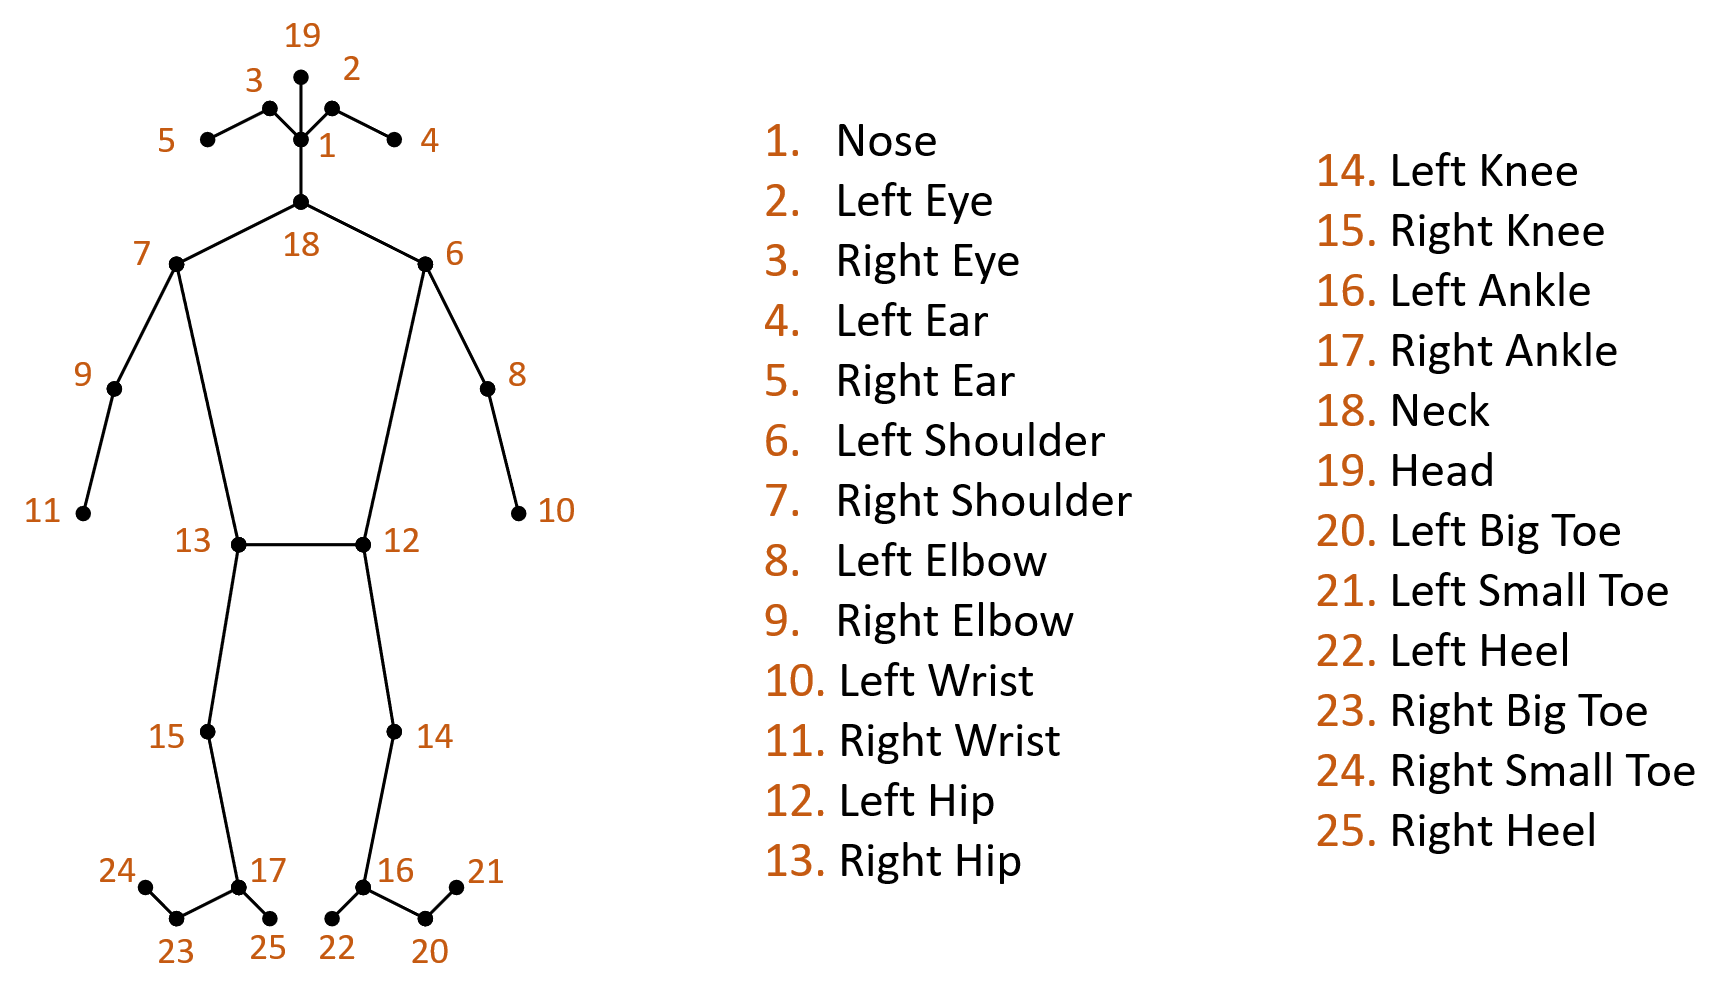
\includegraphics[width=\linewidth]{figure/ch3_fig_OpenPose.png}
    \caption[OpenPose 關節點對應位置]{OpenPose 關節點對應位置}
    \label{ch3_fig_OpenPose}
\end{figure}

\subsection{時間對齊}
% 時間軸對齊介紹
本研究使用拍手~\cite{pons2012data} 的方法進行時間對齊,在實驗動作開始及結束時,受試者皆需進行拍手動作,
動作流程為:兩手打直張開呈現 T pose 維持 1 \textasciitilde\ 2 秒,然後迅速合攏雙手並拍手,最後維持合掌姿勢 1 \textasciitilde\ 2 秒。
透過拍手動作,可在影像資料的音軌中找到明顯的拍手聲音,
並在 IMU 資料中找到快速拍手動作的時間點,因為迅速合攏手掌的拍手動作會產生明顯加速度變化,
以此時間點作為時間對齊的基準點,將影像資料及 IMU 資料進行時間對齊,以確保兩者之間的時間軸一致。
在對齊並剪輯影像資料及 IMU 資料時有一點需要注意,
對齊兩種資訊時,由於加速度的明顯變化是發生在拍手那一刻的前後一幀,
因此在裁切 IMU 資料時,需將拍手動作前後一幀的資料保留,確保拍手動作的加速度變化完整呈現,
進行影像剪輯時,需將合掌姿勢前後一個幀的影像資料保留,以確保拍手動作的完整呈現,且可與 IMU 資料對齊。

\subsection{空間對齊}
% 座標系轉換介紹
在人體量測領域中,每一量測方法都有其固有且常用的座標系,
因此在進行感測器融合時,必須將各感測器的座標系轉換至同一座標系,以方便後續感測器融合計算。
本研究共涉及六種座標系,可分為影像系統及 IMU 感測器系統兩大部分,兩部分的共同座標系為全域座標系 (global coordinate system, g)。
影像系統涉及三種座標系,分別為圖像座標系 (image coordinate system, img)、
相機座標系 (camera coordinate system, cam) 及全域座標系 (global coordinate system, g);
IMU 感測系統則涉及四種座標系,分別為骨骼座標系 (bone coordinate system, b)、感測器座標系 (sensor coordinate system, s)、
IMU local 座標系 (imu local coordinate system, i)、全域座標系 (global coordinate system, g)。
各座標系的定義及轉換關係將於以下進行介紹。

\subsubsection{座標系定義}
% 各座標系定義介紹
圖像座標系為二維座標系,以圖像左上角為原點,x 軸沿圖像右側為延伸為正,y 軸沿圖像下側延伸為正,如圖~\ref{ch3_fig_frame} (a) 所示;
相機座標系以相機的光心為原點,z 軸與光軸重和,指向相機前方為正, x 軸指向相機右方為正, y 軸指向相機下方為正,如圖~\ref{ch3_fig_frame} (b) 所示;
骨骼座標系以 TotalCapture Dataset 提供之 Vicon 三維人體模型所在之座標系為基礎,如圖~\ref{ch3_fig_frame} (c) 所示,
其以人體骨盆中心為原點, +x、+y、+z 方向分別為向右 (red)、向後 (green)、向下 (blue);
感測器座標系,以感測器本身為原點,
於 Xsens 系統中,定義其 x 軸為長邊延伸方向,y 軸為短邊延伸方向,z 軸則沿最大平面法向,
如圖~\ref{ch3_fig_frame} (d) 所示;
IMU local 座標系以感測器所在地為原點,y 軸沿子午線指向正北為正,z 軸指向天頂為正,x 軸與 yz 平面垂直,指向正東為正;
全域座標系以固定的全球基準點為原點 (例如地球中心),x 軸以磁北極為參考方向,z 軸參考方向與 IMU local 座標系 z 軸相同,指向天頂為正,
y 軸則以右手定則決定,通常指向西方為正。
座標系間的關係及旋轉矩陣將於下一段進行介紹。

\begin{figure}[!ht]
   \centering
   \begin{minipage}{.5\textwidth}
      \centering
      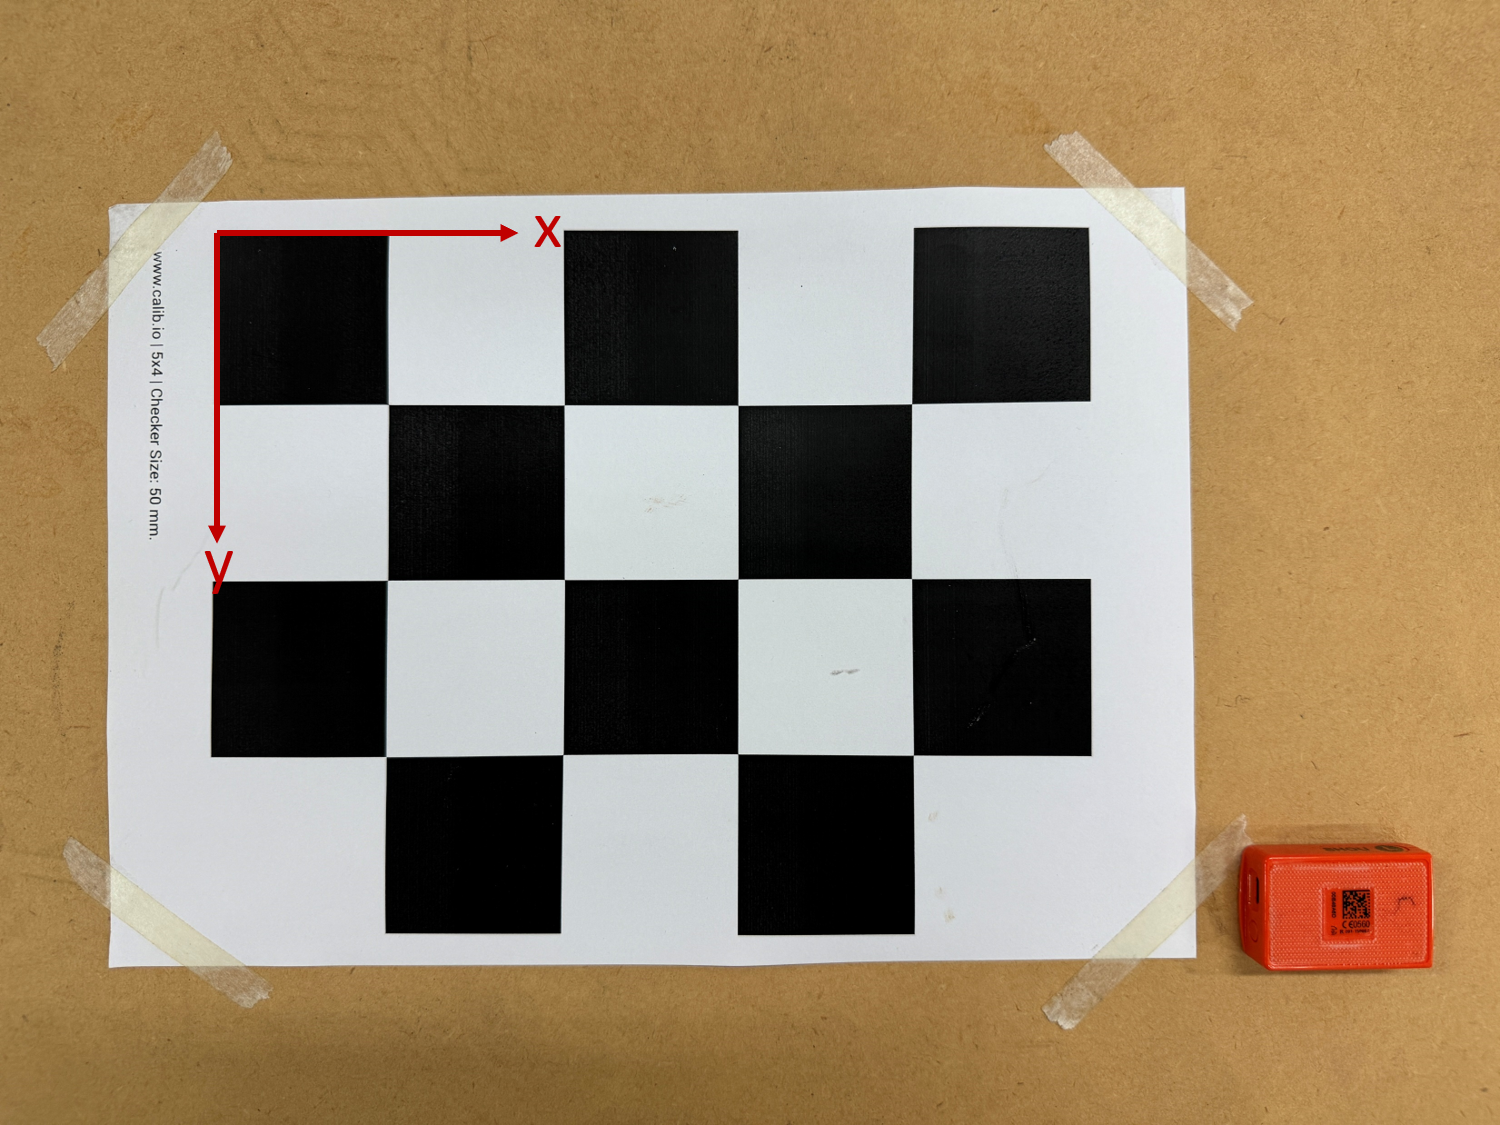
\includegraphics[width=\linewidth]{figure/ch3_fig_imgframe.png}
      \caption*{(a) 影像座標系}
   \end{minipage}%
   \vspace{5mm}%
   \begin{minipage}{.5\textwidth}
      \centering
      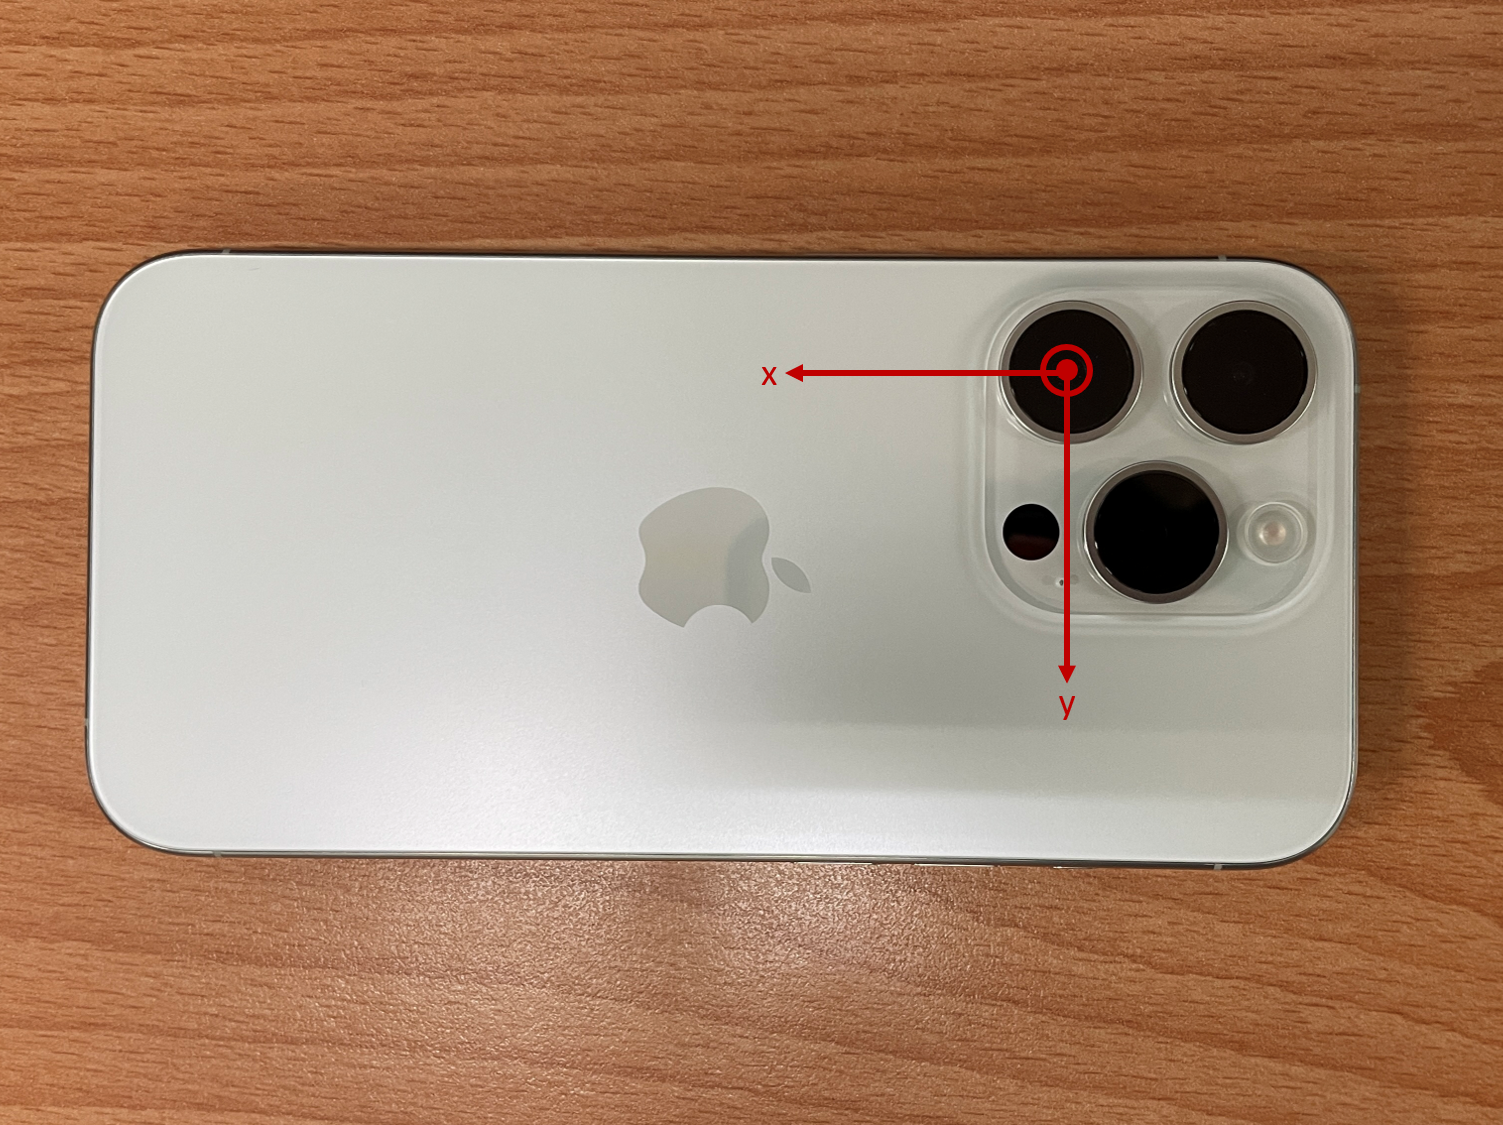
\includegraphics[width=\linewidth]{figure/ch3_fig_camframe.png}
      \caption*{(b) 相機座標系}
   \end{minipage}
   \begin{minipage}{.5\textwidth}
     \centering
     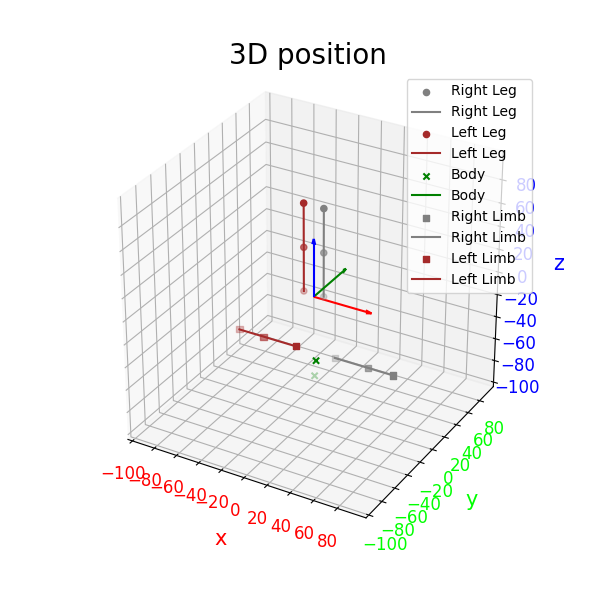
\includegraphics[width=\linewidth]{figure/ch3_fig_skeleton_frame.png}
     \caption*{(c) 骨骼座標系}
   \end{minipage}%
   \begin{minipage}{.5\textwidth}
     \centering
     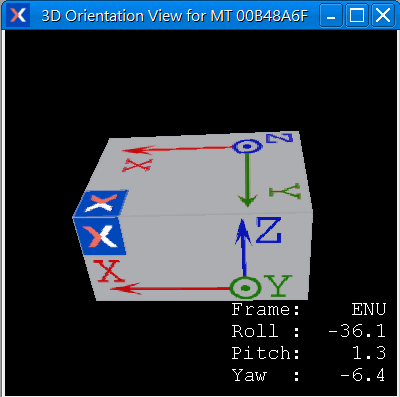
\includegraphics[width=\linewidth]{figure/ch3_fig_imu_frame.png}
     \caption*{(d) 感測器座標系}
   \end{minipage}
   \captionsetup{justification=centering}
   \caption[座標系定義]{座標系定義}
   \label{ch3_fig_frame}
\end{figure}

\subsubsection{各座標系間的關係}
% 各座標系間的關係介紹
在影像系統座標系定義與轉換的部分,本研究使用關係式~\ref{ch3_equ_image_rotation_matrix},
將在空間中的位置點由以全域座標系為表示方式轉換至以相機座標系為表示方式。

\begin{equation}
   R^{cam}_{g} = R^{cam}_{img}(R^{g}_{img})^{-1}
   \label{ch3_equ_image_rotation_matrix}
\end{equation}

其中,$R^{cam}_g$ 為將空間中的位置點由全域座標系轉換至相機座標系之旋轉矩陣,
即圖~\ref{ch3_fig_coordinate_trans} 中,從綠色座標系轉換至紫色座標系之旋轉矩陣,
通過將 $R^{cam}_g$ 乘以全域座標系中的骨骼朝向,將以全域座標系表示之朝向轉換為以相機座標系表示的骨骼朝向;
$(R^{g}_{img})^{-1}$ 為全域座標系轉換至圖像座標系之旋轉矩陣,
即圖~\ref{ch3_fig_coordinate_trans} 中,從綠色座標系轉換至粉色座標系之旋轉矩陣,
通過將 $R^{cam}_g$ 乘以全域座標系中的骨骼朝向,將以全域座標系表示之朝向轉換為以圖像座標系表示的骨骼朝向;
$R^{cam}_{img}$ 為圖像座標系轉換至相機座標系之旋轉矩陣,
即圖~\ref{ch3_fig_coordinate_trans} 中,從粉色座標系轉換至紫色座標系之旋轉矩陣,
通過將 $R^{cam}_{img}$ 乘以圖像座標系中的骨骼朝向,將以圖像座標系表示之朝向轉換為以相機座標系表示的骨骼朝向。

在 IMU 感測器系統座標系定義與轉換的部分,
本研究參考文獻~\cite{malleson2017real}所提出之關係式~\ref{ch3_equ_imu_rotation_matrix},並進行修正以更有助於理解,
將每一關節點由以骨骼座標系為表示方式轉換至以全域座標系為表示方式。

\begin{equation}
   R^g_b=R^g_iR^i_s(R^b_s)^{-1}
   \label{ch3_equ_imu_rotation_matrix}
\end{equation}

其中,$R^g_b$ 為將 IMU 所附著的骨骼朝向由骨骼座標系轉換至全域座標系之旋轉矩陣,
即圖~\ref{ch3_fig_coordinate_trans} 中,從黑色座標系轉換至綠色座標系之旋轉矩陣,
通過將 $R^g_b$ 乘以骨骼座標系中的骨骼朝向,將以骨骼座標系表示之朝向轉換為以全域座標系表示的骨骼朝向;
$(R^b_s)^{-1}$ 為骨骼座標系轉換至感測器座標系之旋轉矩陣,
即圖~\ref{ch3_fig_coordinate_trans} 中,從黑色座標系轉換至紅色座標系之旋轉矩陣,
通過將 $(R^b_s)^{-1}$ 乘以骨骼座標系中的骨骼朝向,將以骨骼座標系表示之骨骼朝向轉換為以感測器座標系表示的骨骼朝向;
$R^i_s$ 為感測器座標系轉換至 IMU local 座標系之旋轉矩陣,
即圖~\ref{ch3_fig_coordinate_trans} 中,從紅色座標系轉換至藍色座標系之旋轉矩陣,
通過將 $R^i_s$ 乘以感測器座標系中的骨骼朝向,將以感測器座標系表示之骨骼朝向轉換為以 IMU local 座標系表示的骨骼朝向;
$R^g_i$ 為 IMU local 座標系轉換至全域座標系之旋轉矩陣,
即圖~\ref{ch3_fig_coordinate_trans} 中,從藍色座標系轉換至綠色座標系之旋轉矩陣,
通過將 $R^g_i$ 乘以 IMU local 座標系中的骨骼朝向,將以 IMU local 座標系表示之骨骼朝向轉換為以全域座標系表示的骨骼朝向。
上述所提及之每一旋轉矩陣的量測與計算方式將於後續進行介紹。

\begin{figure}[!ht]
   \centering
   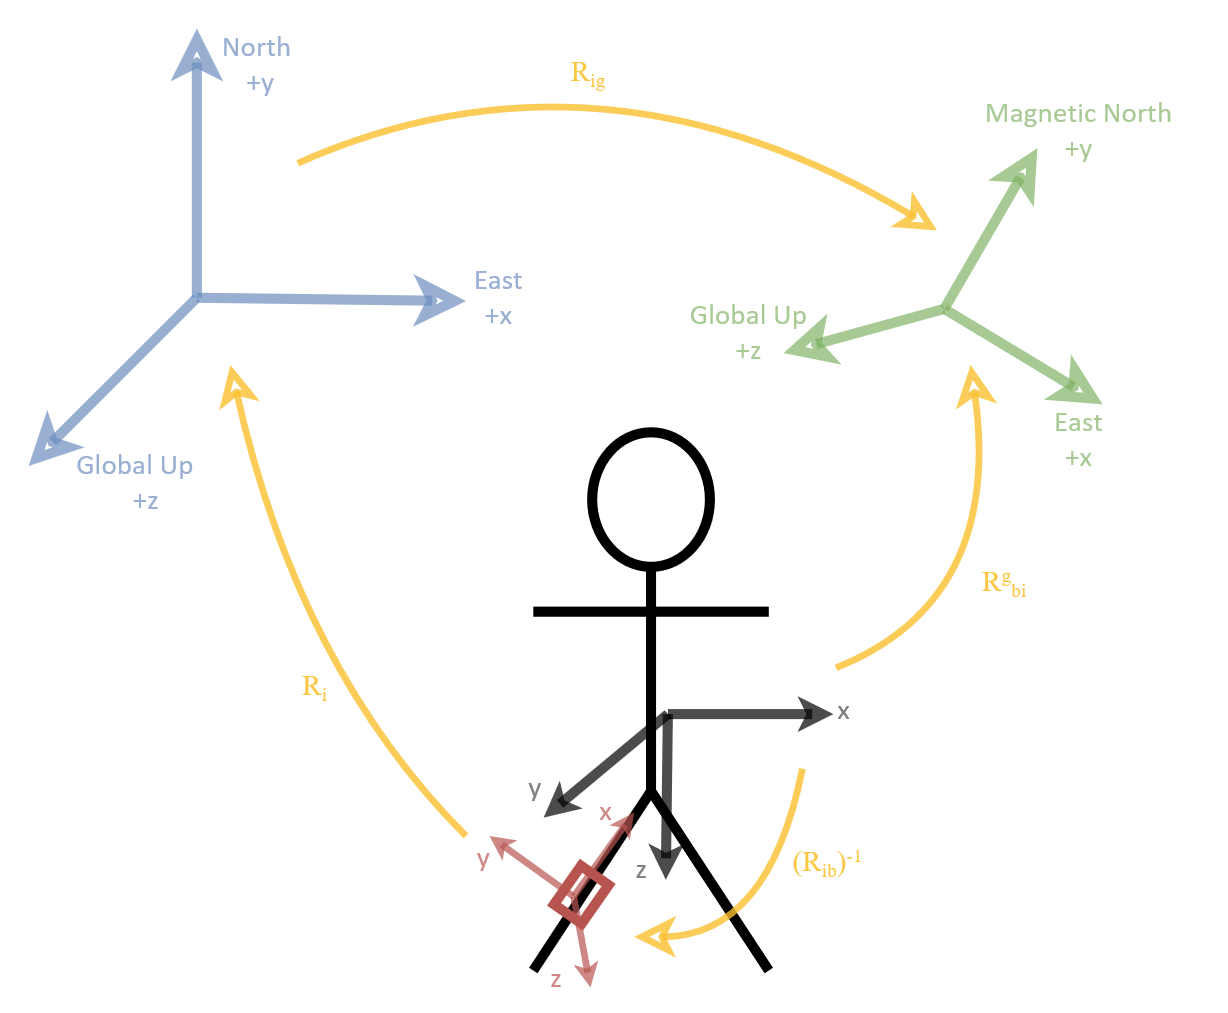
\includegraphics[width=\textwidth]{figure/ch3_fig_coordinate_trans.png}
    \caption[各座標系間的關係]{各座標系間的關係}
    \label{ch3_fig_coordinate_trans}
\end{figure}

\subsubsection{圖像座標 - 全域座標旋轉矩陣,$R^{g}_{img}$}
%圖像座標 - 全域座標旋轉矩陣
圖像座標 - 全域座標旋轉矩陣 ($R^{g}_{img}$) 為計算受試者手上棋盤格校正板與全域座標系間關係之旋轉矩陣,
其可將圖像座標系轉換至全域座標系,
將座標系統一轉換到全域座標系,以方便後續進行感測器融合計算。
圖像座標 - 全域座標旋轉矩陣計算方式如方程式~\ref{ch3_equ_img2g_rotation_matrix} ,
本研究將棋盤格校正板安裝上 IMU,並將棋盤格校正板的 x、y 座標方向與 IMU 的 x、y 對齊,
經過對齊後,IMU 的朝向可直接視為棋盤格校正板的朝向,因此 $R^{i}_{img} = R^{i}_{s}$,
經由 IMU 量得的 IMU - IMU local 旋轉四元數即可視為棋盤格校正板 - IMU local 的旋轉四元數,
再將整體座標系對 y 軸旋轉 $90^{\circ}$ ,對 x 軸旋轉 $180^{\circ}$ ,即可得到圖像座標 - 全域座標旋轉矩陣。

\begin{equation}
   R^{g}_{img} = R_{x}(\theta_{x})R{y}(\theta_{y})R^{i}_{img} = R_{x}(\theta_{x})R{y}(\theta_{y})R^{i}_{s}
   \label{ch3_equ_img2g_rotation_matrix}
\end{equation}

\subsubsection{圖像座標 - 相機座標旋轉矩陣,$R^{cam}_{img}$}
% 圖像座標 - 相機座標旋轉矩陣
圖像座標 - 相機座標旋轉矩陣 ($R^{cam}_{img}$) 為計算受試者手上棋盤格校正板與相機間關係之旋轉矩陣,
其可將圖像座標系轉換至相機座標系,
本研究之計算方式為使用一 5x4,方格寬度為 50 (mm) 的棋盤格校正板,
並使用 Pose2Sim ~\cite{Pagnon_2022_JOSS}~\cite{Pagnon_2021_Robustness}~\cite{Pagnon_2022_Accuracy} 提供的校正工具進行外部參數及內部參數計算,
透過相機校正所得之外部參數即為棋盤格校正板與相機間的旋轉及平移關係。

\subsubsection{感測器座標 - 骨骼座標旋轉矩陣,$R^b_s$}
% IMU - 骨骼座標轉換矩陣計算介紹
% 解釋表示方法是以哪個座標系去看哪個座標系,然後解釋計算方法
使用 IMU 進行肢體朝向量測時,由於 IMU 黏貼於肢體上的方向及位置可能會和骨骼定義之方向及位置有所偏差,
因此需使用感測器座標 - 骨骼座標旋轉矩陣($R^b_s$),將位於感測器座標系的量測數值轉換為以骨骼座標系表示的骨骼朝向。
感測器座標 - 骨骼座標旋轉矩陣計算方式如方程式~\ref{ch3_equ_b2s_rotation_matrix},
假設受試者在最初始開始實驗時,設定一個與 IMU local 座標系對齊的座標系統,且受試者的姿勢為 T pose,
因此此時 IMU 到其附著肢段的旋轉矩陣與 IMU 到 IMU local 的旋轉矩陣相同,即 $R^{b}_{s}(t_0) = R^{i}_{s}(t_0)$,
因此,在 $t_0$ 時刻量得的 IMU - IMU local 旋轉四元數即可視為感測器座標 - 骨骼座標旋轉四元數,
而由於在章節~\ref{ch3_skeleton_method} 中建立的人體模型座標與 IMU 附著於骨骼定義的座標系相差 $180^{\circ}$,
因此,再將整體座標系對 x 軸旋轉 $180^{\circ}$ ,即可得最終感測器座標 - 骨骼座標旋轉矩陣。 

\begin{equation}
   R^{b}_{s} = R_{x}(\theta_{x})R^{b}_{s}(t_0) = R_{x}(\theta_{x})R^{i}_{s}(t_0)
   \label{ch3_equ_b2s_rotation_matrix}
\end{equation}

% 此矩陣可經由 OpenSim~\cite{delp2007opensim}處理並進一步計算而得,其取得及計算方式如下。
% 首先,量測結束之 IMU 資料將透過 OpenSim 軟體進行處理,\sout{使用基礎骨骼模型...},計算每一 IMU 相對其對應骨骼之相對位置及角度,
% 處理結果可經由 OpenSim 軟體可視化,如圖~\ref{ch3_fig_imu_ori} 所示。
% 此項數據紀錄於 OpenSim 輸出之 .osim 檔案的 <BodySet> 元素中,<BodySet> 以骨骼為單位,
% 其中包含之 <components> 則記錄一附著於該骨骼上之 IMU 的相對位置及角度,
% <translation> 代表該 IMU 的原點相對於其附著之骨骼原點的平移,
% <orientation> 則代表該 IMU 的座標軸相對於其附著之骨骼坐標軸的旋轉。
% 因此若將 <translation> 數值更改為零,則可看到 IMU 原點與骨骼原點重合,如圖~\ref{ch3_fig_imu_tra},
% 而若將 <orientation> 數值更改為零,則可看到 IMU 坐標軸與骨骼坐標軸平行,如圖~\ref{ch3_fig_imu_rot}。
% 因此,從 .osim 檔案取得每一 IMU 相對於骨骼之相對位置及角度後,即可計算出感測器座標 - 骨骼座標四元數。
% \begin{figure}[!ht]
%    \centering
%    \begin{minipage}{.3\textwidth}
%      \centering
%      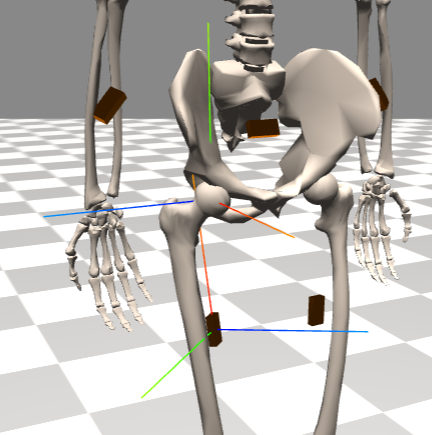
\includegraphics[width=.8\linewidth, height=.8\linewidth]{figure/ch3_fig_imu_ori.png}
%      \caption[OpenSim 計算結果]{OpenSim 計算結果}
%      \label{ch3_fig_imu_ori}
%    \end{minipage}%
%    \begin{minipage}{.3\textwidth}
%      \centering
%      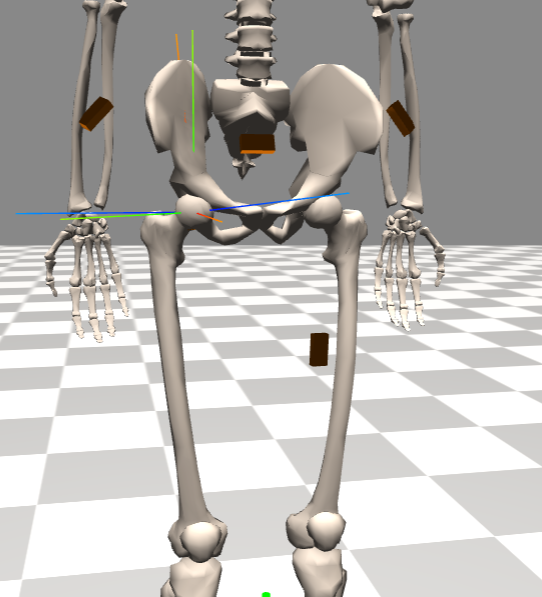
\includegraphics[width=.8\linewidth, height=.8\linewidth]{figure/ch3_fig_imu_tra.png}
%      \caption[IMU 平移為零]{IMU 平移為零}
%      \label{ch3_fig_imu_tra}
%    \end{minipage}%
%    \begin{minipage}{.3\textwidth}
%       \centering
%       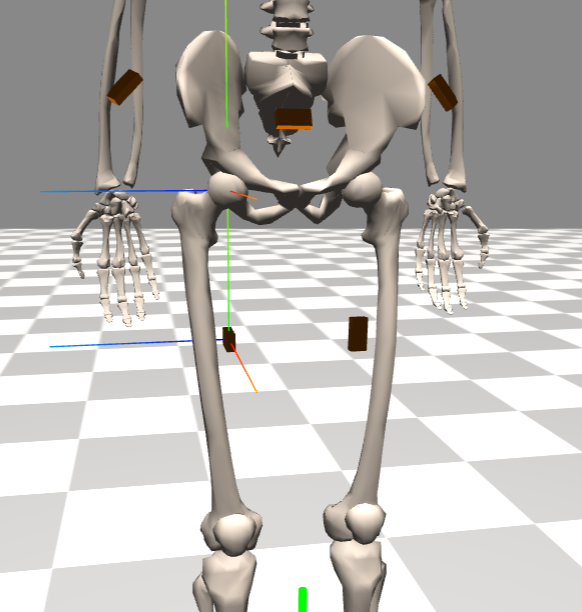
\includegraphics[width=.8\linewidth, height=.8\linewidth]{figure/ch3_fig_imu_rot.png}
%       \caption[IMU 旋轉為零]{IMU 旋轉為零}
%       \label{ch3_fig_imu_rot}
%     \end{minipage}
% \end{figure}

\subsubsection{感測器座標 - IMU local 旋轉矩陣,$R^i_s$}
經過上一步 $(R^b_s)^{-1}$ 的轉換,已將骨骼朝向轉換為以附著其上的 IMU 感測器座標系為表示方式,
接著,需要進一步將各自表示的感測器座標系轉換至統一以東北天 (East - North - Up, ENU) 為定義的 IMU local 座標系。
感測器座標 - IMU local 旋轉矩陣 ($R^i_s$) 為 IMU 的量測朝向,可直接經由 Xsens 系統所提供軟體 (MT manager) 輸出四元數取得。
在 MT manager 中讀入量測時所記錄的 .mtb 檔案,
% TODO:...模型為基礎
並於 file>export 中的輸出選項勾選 quaternion 後輸出,
每一 .txt 檔案中的 q0、q1、q2、q3 即為將朝向旋轉乘以 IMU local 座標系為表示方式的旋轉四元數,分別代表四元數的 w、x、y、z,
將四元數轉換為旋轉矩陣即可得感測器座標 - IMU local 旋轉矩陣。

\subsubsection{IMU local - 全域座標旋轉矩陣,$R^g_i$}
% IMU - 全域座標轉換矩陣計算介紹
% 解釋表示方法是以哪個座標系去看哪個座標系,然後解釋計算方法
經過上一步 $R^i_s$ 的轉換,已將骨骼朝向轉換為以統一的 IMU local 感測器座標系為表示方式,
接著,為方便後續與影像辨識而得的位置資訊進行融合,需要進一步將骨骼朝向轉換至位置資訊所在之座標系。
假設所有 IMU 間的 IMU local - 全域座標旋轉矩陣 $R^g_i$ 皆一致,且與天頂及磁北極對齊,
再將整體座標系相對 x 軸旋轉 $-90^{\circ}$,即可得 IMU local - 全域座標旋轉矩陣。
% 包含兩個階段的旋轉,
% 第一階段先將於 IMU local 座標系的骨骼朝向轉換至以全域座標系表示,與天頂及磁北極對齊,
% 第二階段將於全域座標系的骨骼朝向轉換至位置資訊所在之座標系,該座標系相對全域座標系的 x 軸旋轉 $-90^{\circ}$。
% 在第一階段中,IMU local - 全域座標的轉換與磁偏角 ($\delta$) 有關,
% 將 IMU local 座標系繞 z 軸旋轉 $\delta$ 即可轉換至全域座標系。
% 第二階段再將全域座標系繞 x 軸旋轉 $-90^{\circ}$,轉換至位置資訊所在之座標系。

% ------------------------- 3.3 ------------------------- %
\section{感測器融合方法}
% 感測器融合方法介紹
% 這邊如果篇幅過大也可以另立成3.3,cameraset 就改成 3.4
IMU image pytorch

% ------------------------- 3.4 ------------------------- %
\section{探討減少相機數量的可行性}
% 探討減少相機數量的可行性及其擺放位置介紹,可是擺放位置的結論還沒有可以很好的呈現方式,所以暫時先不要有這方面的結論和討論
% FIXME:可以從增加實驗架設方便性方面作為開頭著手,然後這邊應該可以算是解釋為何我要用兩台相機,所以位置可能需要改到第三章的最一開始,補充 total 還有提供完整的相機、IMU、vicon 資料,可以方便的直接開始進行探討
TotalCapture Dataset~\cite{Trumble:BMVC:2017}提供 8 台相機與 13 個 IMU 的量測資料,
而在文獻~\cite{Zhang_2020_CVPR}中,作者使用到 4 台相機及 8 個 IMU 的資料;
% 另外在 TotalCapture Dataset 發表的文獻~\cite{Trumble:BMVC:2017}中則有提及嘗試減少相機的硬體數量,準確度隨著相機數量的減少而下降,
因此本章節嘗試以減少相機數量\sout{並選擇相機擺放位置}進行感測器融合計算的方式,
探討減少相機使用數量對於動作捕捉的影響,\sout{並嘗試探討相機擺放位置的選擇}。

\subsection{實驗方法}
% 實驗方法介紹
% 目前的相機用量及擺放位置敘述,要 cite totalcapture 和 data fusion
TotalCapture Dataset 實驗環境為一個 4x6 (m) 的方形空間,每一面牆面上方架設兩台相機,
四面牆共計八台相機,每台相機距離地面高度皆為 2.5 (m),擺放位置以上視的視角呈現,如圖~\ref{ch3_fig_cameraset_totalcap} 所示。
本次實驗將分成七類情況進行,第一類情況為從八台相機中任選一台相機進行感測器融合計算,
並將得到的姿勢估計結果與 TotalCapture Dataset 提供的 Vicon 位置資料進行比對,計算平均每關節誤差 (mean per joint position error, MPJPE),
第二類為任選兩台相機進行姿勢估計,以此方式遞增至第七類,任選七台相機進行姿勢估計,每一類情況皆會產生一組 MPJPE。

\begin{figure}[!ht]
   \centering
   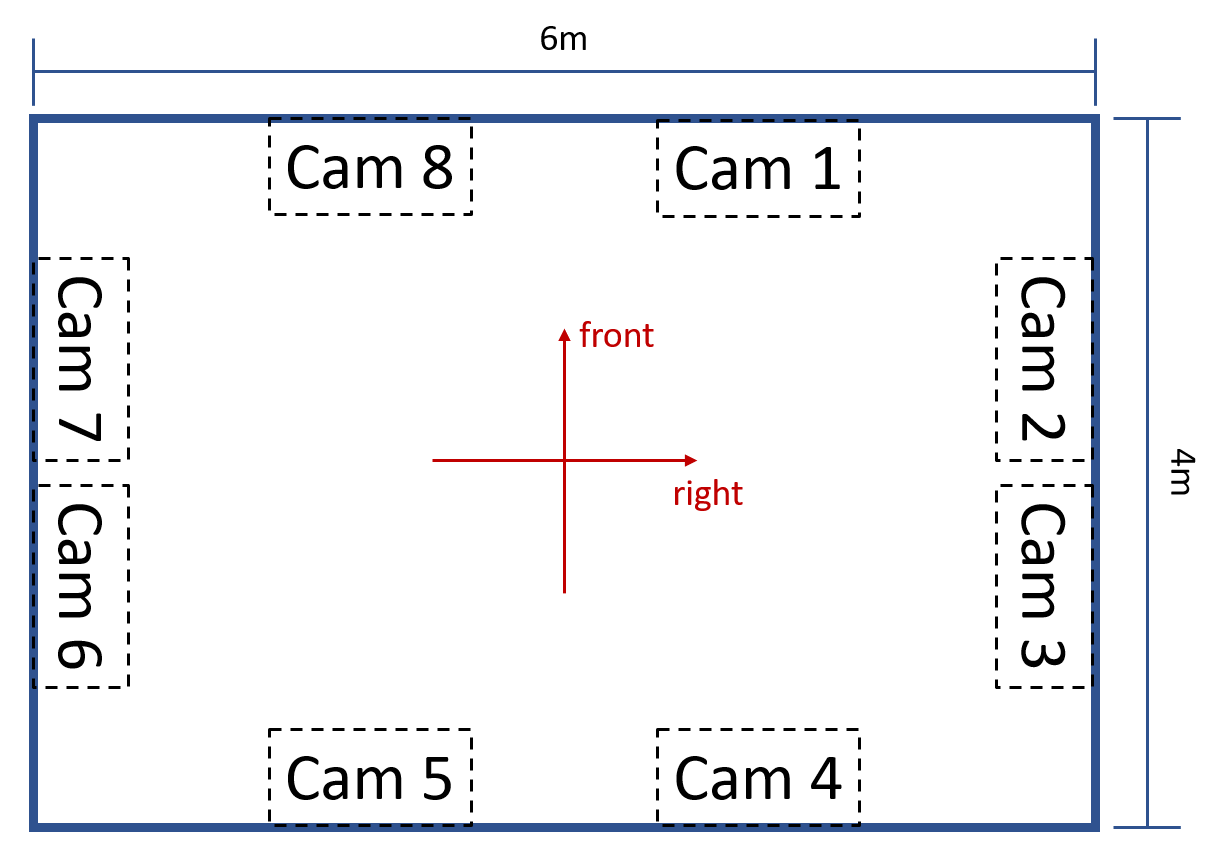
\includegraphics[width=8cm]{figure/ch3_fig_cameraset_totalcap.png}
    \caption[相機擺放位置]{相機擺放位置}
    \label{ch3_fig_cameraset_totalcap}
\end{figure}

% ------------------------- 3.4 ------------------------- %
\section{結果可視化}
% 結果可視化介紹
% 分類成五個部分,分別用甚麼顏色表示

% ------------------------- 3.5 ------------------------- %
\section{小結}
% 本章架構
本章節首先介紹將會使用到的背景知識,像是透過希爾式肌肉模型來模擬肌肉,藉此理解肌肉的機械與生理特性,
而藉由 OpenSim 的協助,不但能快速建立肌肉骨骼模型,還可以執行正向動力學與肌肉計算控制等模擬,
且得到一個可信的結果,接下來介紹本研究的核心模擬——運動軌跡預測任務,後續的敏感度分析、最佳化過程與模型驗證,
皆是以預測任務為基礎來延伸,透過預測任務來檢視模型的表現,亦即預測誤差。
本研究透過敏感度分析來得知肌肉與任務之間的關係,藉此挑選合適的任務集作為參數評估輸入,
搭配最佳化演算法來進行參數估計,其中多組預測任務具有讓目標函數更加明確的功用,避免參數不具識別性的原因,
掉入至局部最小值結果當中,最終透過間接方法來驗證模型的正確性。

% 應用
該研究方法之應用可分為兩種討輪,第一是模擬研究,即為本研究使用之方法,透過純模擬研究來檢視該方法的可行性,
優點是其具有明確答案可供參考,且無需考慮量測造成的不確定性,在進入到實際應用前,也必須先確認模擬研究是可執行的;
第二種則是實際應用,其可透過 EMG 與動作捕捉系統來達成,藉由 EMG 量測肌肉訊號作為輸入,
動作捕捉系統量測運動軌跡作為輸出之結果比較,兩者結合並搭配本研究之最佳化方法,即可達成肌肉之參數估計,
但存在龐大的量測不確定性情況下,由於微小的軌跡偏離,即會造成肌肉參數的變動與抗衡,
縱使估計出肌肉參數,其結果之正確性仍有待商榷,因此於現今之科技發展,要達成實際應用仍有一段距離。

% 下一章節
本章節主要介紹論文之研究方法,下章節會以實際模型與動作進行討論,藉由上方所提及之方法與流程,
針對模型進行肌肉參數評估的前置作業與套用說明。

\clearpage